\documentclass[twoside,11pt]{book}
% preambulo
\usepackage[utf8]{inputenc}
\usepackage{lmodern}
\usepackage[T1]{fontenc}
\usepackage[spanish,activeacute,es-tabla]{babel}
\usepackage{mathtools} 
\usepackage{titlesec}
\usepackage{eurosym}

\usepackage{amssymb, amsmath, amsbsy} % simbolitos
\usepackage{upgreek} % para poner letras griegas sin cursiva
\usepackage{cancel} % para tachar
\usepackage{mathdots} % para el comando \iddots
\usepackage{mathrsfs} % para formato de letra
\usepackage{stackrel} 

% tamaño de las páginas y ejes
\usepackage{vmargin}
\setlength{\oddsidemargin}{37mm}
\setlength{\evensidemargin}{30mm}
\setlength{\headsep}{1.2cm}
\setlength{\textwidth}{143mm}
\setlength{\textheight}{225mm}
\setlength{\topmargin}{30mm}
\setlength{\headheight}{0mm}

% Tamaño de los parrafos
\setlength{\parskip}{0.5cm}
\setlength{\parindent}{1cm}

% Estilo del titulo de página
\pagestyle{headings}
\markboth{CAP'ITULO 1}{INTRODUCCI'ON}

% enumerados
\usepackage{enumerate}

% Tablas
\usepackage{multirow}
\usepackage{longtable} % tablas largas
\usepackage{rotating} % rotar tablas

%color
\usepackage[usenames]{color}

%Algoritmos
\usepackage{algorithmic}
\usepackage{verbatim}
\usepackage{listings}

%document

\usepackage{cite}
\usepackage[backref=false]{hyperref}

%graficos
\usepackage{graphicx}
\usepackage{subfigure}


\usepackage{listingsutf8}
\lstset{ frame=Ltb,
framerule=0pt,
aboveskip=0.5cm,
framextopmargin=3pt,
framexbottommargin=2.5pt,
framexleftmargin=0cm,
framesep=0pt,
rulesep=.4pt,
backgroundcolor=\color{gray97},
rulesepcolor=\color{black},
%
stringstyle=\ttfamily,
showstringspaces = false,
basicstyle=\small\ttfamily,
commentstyle=\color{gray45},
keywordstyle=\upshape\bfseries\ttfamily\large\color{blue},
%
numbers=none,
numbersep=15pt,
numberstyle=\tiny,
numberfirstline = false,
breaklines=true,
breakindent=0pt,
showtabs=false,
%
mathescape=true,
%
literate=
    {á}{{\'a}}1 {é}{{\'e}}1 {í}{{\'i}}1 {ó}{{\'o}}1 {ú}{{\'u}}1
    {Á}{{\'A}}1 {É}{{\'E}}1 {Í}{{\'I}}1 {Ó}{{\'O}}1 {Ú}{{\'U}}1
    {à}{{\`a}}1 {è}{{\`e}}1 {ì}{{\`i}}1 {ò}{{\`o}}1 {ù}{{\`u}}1
    {À}{{\`A}}1 {È}{{\'E}}1 {Ì}{{\`I}}1 {Ò}{{\`O}}1 {Ù}{{\`U}}1
    {ä}{{\"a}}1 {ë}{{\"e}}1 {ï}{{\"i}}1 {ö}{{\"o}}1 {ü}{{\"u}}1
    {Ä}{{\"A}}1 {Ë}{{\"E}}1 {Ï}{{\"I}}1 {Ö}{{\"O}}1 {Ü}{{\"U}}1
    {â}{{\^a}}1 {ê}{{\^e}}1 {î}{{\^i}}1 {ô}{{\^o}}1 {û}{{\^u}}1
    {Â}{{\^A}}1 {Ê}{{\^E}}1 {Î}{{\^I}}1 {Ô}{{\^O}}1 {Û}{{\^U}}1
    {œ}{{\oe}}1 {Œ}{{\OE}}1 {æ}{{\ae}}1 {Æ}{{\AE}}1 {ß}{{\ss}}1
    {ç}{{\c c}}1 {Ç}{{\c C}}1 {ø}{{\o}}1 {å}{{\r a}}1 {Å}{{\r A}}1
    {€}{{\EUR}}1 {£}{{\pounds}}1
}

\definecolor{lightyellow}{rgb}{1,1,0.88}
\definecolor{lavanda2}{rgb}{0.9,0.9,0.98}
\definecolor{lavanda3}{rgb}{1,0.94,0.96}
\definecolor{maroon}{rgb}{0.55,0.27,0.07}
\definecolor{gray75}{gray}{.75}
\definecolor{gray97}{gray}{.97}
\definecolor{gray45}{gray}{.45}

% minimizar fragmentado de listados
\lstnewenvironment{listing}[1][]
{\lstset{#1}\pagebreak[0]}{\pagebreak[0]}

\lstdefinestyle{macros}{
language=C,
basicstyle=\upshape\small\ttfamily,
backgroundcolor=\color{lightyellow},
commentstyle =\slshape\bfseries\color{gray45},
emph={[3]size\_t,*,}, emphstyle={[3]\upshape\bfseries\ttfamily\large\color{blue}},
}

\lstdefinestyle{estructura}{
language=C,
basicstyle=\upshape\small\ttfamily,
backgroundcolor=\color{lavanda2},
commentstyle =\slshape\bfseries\color{gray45},
emph={[3]size\_t,*,}, emphstyle={[3]\upshape\bfseries\ttfamily\large\color{blue}},
}

\lstdefinestyle{funcion}{
language=C,
basicstyle=\upshape\small\ttfamily,
backgroundcolor=\color{lavanda3},
otherkeywords={void,*},
commentstyle =\slshape\bfseries\color{gray45},
emph={[1]escribir\_objeto,solicitar_objeto,extraer_temperatura,calcular_error,calcular_tempcontrol,seleccionar_setpoint,enviar_datos,obtener_comando,modular_comando,transmitir_comando,iteracion,modular_bit ,@param}, emphstyle={[1]\upshape\bfseries\ttfamily\large\color{red}},
emph={[2]static,@return}, emphstyle={[2]\itshape\bfseries\ttfamily\large\color{maroon}},
emph={[3]size\_t,*}, emphstyle={[3]\upshape\bfseries\ttfamily\large\color{blue}},
}

\lstdefinestyle{pseudocodigo}{
language=C,
basicstyle=\upshape\small\ttfamily,
backgroundcolor=\color{gray97},
otherkeywords={void,*},
commentstyle =\slshape\bfseries\color{gray45},
emph={[1]escribir\_objeto,solicitar_objeto,extraer_temperatura,calcular_error,calcular_tempcontrol,seleccionar_setpoint,enviar_datos,obtener_comando,modular_comando,transmitir_comando,iteracion,modular_bit ,@param}, emphstyle={[1]\upshape\bfseries\ttfamily\large\color{red}},
emph={[2]static,@return}, emphstyle={[2]\itshape\bfseries\ttfamily\large\color{maroon}},
emph={[3]size\_t,*}, emphstyle={[3]\upshape\bfseries\ttfamily\large\color{blue}},
}

\lstdefinestyle{C}
{language=C,
}

\lstdefinestyle{matlab}
{language=matlab,
}

%Listas
\usepackage{enumerate}

%color para algoritmos
\usepackage{fancyvrb}

% tablas
\usepackage{multirow} 
\usepackage{tabulary}
\usepackage{slashbox} % dibujar diagonales

\setcounter{secnumdepth}{3} % para que ponga 1.1.1.1..
\setcounter{tocdepth}{4} % para que añadir las secciones en el índice...


\usepackage{epstopdf}

\usepackage{float}


\begin{document}
        \frontmatter
        \newpage
            % para comenzar la numeracion de paginas en numeros romanos\begin{flushright}
	
\cleardoublepage
\chapter*{}
\markboth{}{}
\thispagestyle{empty}
\begin{flushright}
\textit{Dedicado a mis padres,\\
mi hermano\\
y mi abuela.\\}
\end{flushright}
        \cleardoublepage
\chapter*{Agradecimientos} % si no queremos que añada la palabra "Capitulo"
\addcontentsline{toc}{chapter}{Agradecimientos} % si queremos que aparezca en el índice
\markboth{}{} % encabezado
 
En primer lugar, quiero dar las gracias a todos los compañeros de \textit{GreenLSI} por haber compartido estos meses de trabajo con vosotros y por vuestra ayuda. En especial a mi tutor Jose Manuel, por haberme guiado en estos meses para sacar adelante este trabajo  y que pudiera ver la luz.

También me gustaría dar las gracias a todos los compañeros que he conocido en todo este tiempo pero sobretodo a Yaiza y Felipe. Gracias por acompañarme hasta el final y por haberme dado muy buenos momentos. Me llevo un grato recuerdo de vosotros.

En este agradecimiento no podrían faltar mis padres y mi hermano, sin los cuales yo no estaría escribiendo estas palabras. Me habeís apoyado y animado desde el inicio y a pesar de las dificultades, habeís seguido apoyándome y confiando en mi, dándome todo lo necesario para que pudiera alcanzar mi objetivo.

Tampoco podían faltar mis amigas Rebeca, Estela, Mari, Emma, Alba, Ana y Marta. Gracias por estar ahí siempre y por tener tantas ganas de verme terminar la carrera. 

No podría terminar este agradecimiento sin darte las gracias a ti, abuela. Este trabajo va dedicado a ti. Por todo el tiempo que esta carrera me ha hecho pasar en tu casa, aguantarme durante los días malos y haberme hecho más ameno esas largas tardes de estudio. Siento que no pueda estar escribiendo estas palabras junto a ti, pero se que me estarás viendo y estarás muy contenta de que a pesar de todas las dificultades, he conseguido llegar a mi objetivo.


	\cleardoublepage
\chapter*{Resumen} % si no queremos que añada la palabra "Capitulo"
\addcontentsline{toc}{chapter}{Resumen} % si queremos que aparezca en el índice
\markboth{}{} % encabezado

	Este trabajo fin de grado (TFG) presenta el diseño e implementación de un sistema de actuación con el que se pueda controlar la refrigeración de una sala de servidores o de un centro de datos (CPD).

	En este trabajo se pretende dar soporte a un sistema de monitorización y optimización energética de centros de datos y poder aplicar una de sus optimizaciones que está basada en el sistema de refigeración. El sistema de optimización, mediante un algoritmo, predice la temperatura a la que debe estar una sala de servidores para que el consumo energético de dicha sala sea mínimo. Para lograr este objetivo, es necesario actuar sobre el sistema de refrigeración y regular su temperatura de funcionamiento de forma dinámica. De este modo, se consigue que la sala alcance el valor de temperatura deseado.

	Teniendo en cuenta esta necesidad, se ha diseñado e implementado un sistema de actuación basado en un sistema de control en lazo cerrado. Se ha conseguido que el sistema sea capaz de regular la temperatura de la sala, siguiendo el valor de temperatura óptima proporcionada por el algoritmo. Este sistema obtiene los datos de temperatura desde una plataforma web, en tiempo real y sin necesidad de ningún tipo de acción humana. También se ha conseguido que el sistema sea dinámico y capaz de responder a las distintas variaciones que puedan producirse en la temperatura óptima, de una forma estable y con la mayor rapidez posible. El sistema de control utilizado se basa en un controlador PID, que posee una implementación sencilla y proporciona un amplio rango de operación, además de que es ampliamente usado en la industria para el control de procesos, incluyendo la temperatura.

	Este sistema de actuación ha sido probado en la sala de servidores B039 del departamento de Ingeniería Electrónica y posteriormente será integrado en el sistema de monitorización y optimización energética desarrollado por el grupo \textit{GreenLSI}, perteneciente a este departamento.

\noindent\textbf{Palabras clave} 

\noindent Centro de procesamiento de datos, sistema de control, optimización energética, control de la temperatura, controlador PID, actuador, sistema ciber-físico, sistema de monitorización.


	\cleardoublepage
\chapter*{Abstract} % si no queremos que añada la palabra "Capitulo"
\addcontentsline{toc}{chapter}{Abstract} % si queremos que aparezca en el índice
\markboth{}{} % encabezado

	This final project work shows the design and implementation of an actuator to control the cooling system of a server room or data center.

	The objective of this work is to apply one type of energy optimization based on the cooling system. An energy monitoring and optimization system predicts what is the optimal temperature of the server room so that the energy consumption is minimum. To apply this optimization, it is necessary to modify dynamically the setpoint of the cooling system to achieve that the temperature of the room reaches the optimal temperature.

	For this reason, an actuator based on a closed loop control system has been designed and implemented. This actuator is capable to setting the optimal temperature in the server room or data center. The actuator obtains the temperature data connecting to a web plataform, in a automatic way and in real time. Also, the actuator is capable of responding to any type of optimum temperature in a dynamic, stable and fast way. The control system used by the actuator is based on a PID controller, which has a simple implementation and provides a wide range of operations. Besides, this type of controller is common used in the industry to process control, including the temperature.

	This actuator has been tested in a server room of the Electronic Engineering Department of Universidad Politécnica de Madrid. Later, this actuator will be integrated in the energy monitoring and optimization system developed by this group.

\noindent\textbf{Keywords}

\noindent Data centers, control system, actuator, energy optimization, temperature control, PID controller, Cyber-Physical System, monitoring system.




	\chapter*{Lista de acrónimos}\label{acronimos}
\addcontentsline{toc}{chapter}{Lista de acrónimos} % para que aparezca en el indice 
\markboth{}{}


\normalsize

\noindent\textbf{BJT} \textit{Bipolar Junction Transistor}

\noindent\textbf{CE} \textit{Chip Enable}

\noindent\textbf{CPD} Centro de Procesamiento de Datos 

\noindent\textbf{CPU} Unidad de Procesamiento de Datos - \textit{Central Processor Unit}

\noindent\textbf{DCIM} \textit{Data Center Infrastructure Management}

\noindent\textbf{DIE} Departamento de Ingeniería Electrónica 

\noindent\textbf{DPM} \textit{Dynamic Power Management} 

\noindent\textbf{DVFS} \textit{Dynamic Voltage Frecuency Scalling}

\noindent\textbf{ETSIT} Escuela Técnica Superior de Ingenieros de Telecomunicación 

\noindent\textbf{GPIO} \textit{General Purpose Input/Output} 

\noindent\textbf{HTTP} Protocolo de Transferencia de Hipertexto - \textit{HyperText Transfer Protocol}

\noindent\textbf{IRLED} \textit{Infrared Light-Emitting Diode} 

\noindent\textbf{IT} \textit{Information Technology} 

\noindent\textbf{JSON} \textit{JavaScript Object Notation} 

\noindent\textbf{KHz} KiloHercio - \textit{KiloHertz} 

\noindent\textbf{LSI} Laboratorio de Sistemas Integrados 

\noindent\textbf{MISO} \textit{Master Input Slave Output}

\noindent\textbf{MOSI} \textit{Master Output Slave Input}

\noindent\textbf{NRMSE} \textit{Normalized Root Mean Square Error} 

\noindent\textbf{PD} Proporcional Derivativo - \textit{Proportional-Derivative}

\noindent\textbf{PI} Proporcional Integral - \textit{Proportional-Integral}

\noindent\textbf{PID} Proporcional Integral Derivativo - \textit{Proportional-Integral-Derivative} 

\noindent\textbf{PUE} \textit{Power Usage Effectiveness} 

\noindent\textbf{SCADA} \textit{Supervisory Control and Data Acquisition} 

\noindent\textbf{SCLK} \textit{Serial Clock} 

\noindent\textbf{SPI} \textit{Serial Peripheral Interface}

\noindent\textbf{TIC} Tecnologías de la Información y Comunicación

\noindent\textbf{TWh} Teravatio-hora - \textit{Terawatt hour}

\noindent\textbf{UPM} Universidad Politécnica de Madrid 

\noindent\textbf{URL} Localizador de Recursos Uniforme  - \textit{Uniform Resource Locator}

\noindent\textbf{VM} Máquina Virtual - \textit{Virtual Machine}

\noindent\textbf{VOVO} \textit{Vary-On Vary-Off}

\noindent\textbf{ZB} {Zettabyte}

        \cleardoublepage
        \tableofcontents % indice de contenidos

	\cleardoublepage
	\addcontentsline{toc}{chapter}{Índice de figuras} % para que aparezca en el indice de figuras
	\listoffigures % indice de figuras

	

        \mainmatter 
    
        \clearpage
	\chapter{Introducci'on}\label{cap:intro}
\normalsize
\thispagestyle{plain}

	Los centros de procesamiento de datos (CPD) son uno de los elementos m'as importantes de Internet ya que almacenan, gestionan y procesan la informaci'on que se mueve a trav'es de la red. Durante los 'ultimos a'nos se ha producido un notable incremento en el uso de las Tecnolog'ias de la Informaci'on y Comunicaci'on (TIC), lo que ha originado un aumento del n'umero, rendimiento y capacidad de almacenamiento de los CPDs. En 2014, las empresas EMC e IDC elaboraron un informe \cite{EMC} que sostiene que el tama'no del universo digital en 2013 fue de 4,4 ZB de informaci'on y estima que dicha cifra se incrementará cada a'no, alcanzando en 2020 los 44ZB de informaci'on, un tama'no 10 veces superior al del 2013.
	
	Esta tendencia implica que los CPDs cada vez tendr'an que procesar, almacenar y gestionar m'as informaci'on en el futuro debido al despliegue de nuevo servicios (\textit{cloud computing, IOT, smartcities, e-health...}). Al tener que manejar un mayor volumen de informaci'on, su infraestructura ser'a cada vez m'as grande y tendr'a un mayor n'umero de equipos (servidores, routers, switches, equipos de refrigeraci'on e iluminaci'on...), lo que har'a que su consumo se incremente. En 2014, un informe elaborado por la empresa Yole D'eveloppement \cite{yole} muestra que el consumo de energ'ia mundial de todos los CPDs en ese a'no fue de 352.4 TWh, que equivale al 1.6\% del consumo mundial de energ'ia de ese año, y concluye que si se mantiene esta tendencia, el consumo en 2020 será aproximadamente de 507.9 TWh, lo que supone un incremento del 25\%.

	Todo esto supone un gran impacto econ'omico y medioambiental, por lo que es necesario aplicar medidas que permitan que los centros de datos operen de una forma m'as eficiente y reduzcan su consumo el'ectrico. Para contextualizar correctamente este problema, primero es necesario conocer cómo se distribuye el consumo en un CPD y cómo se mide su eficiencia. Una vez se conoce la distribución del consumo, se van a mencionar las técnicas que se utilizan para reducirlo. Por último, se exponen las soluciones que existen actualmente para tratar este problema y se enfoca el papel de este TFG en dicha solución.

\section{Eficiencia energ'etica en los centros de datos}\label{sec.situacionactual}

	En la figura \ref{fig1_1:cons} se muestran 2 gr'aficos que representan la distribuci'on del consumo de un CPD t'ipico, realizados   por Rychard L. Sawyer \cite{consumo1} y la empresa EYP Mission Critical Facilities \cite{consumo2}, respectivamente. Ambos gr'aficos difieren en el porcentaje y en c'ual es el tipo de infraestructura que m'as consume. Sin embargo, ambos coinciden en que los equipos IT y la refrigeraci'on son los 2 tipos de infraestructura que m'as potencia consumen dentro del CPD, llegando a usar m'as del 75-80\% de la potencia total.

\begin{figure}[htbp]
  \raggedright
	\subfigure{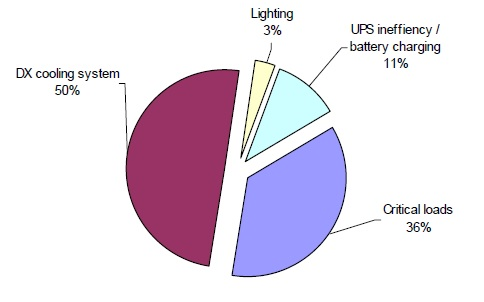
\includegraphics[width=70mm, height=47mm]{imagenes/capitulo1/1_1AConsumo}}
 	\subfigure{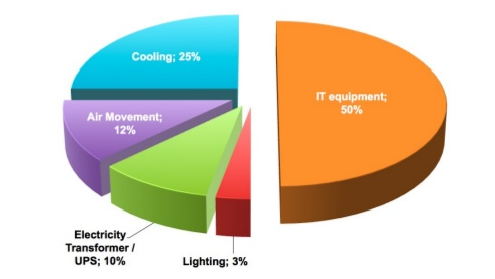
\includegraphics[width=70mm, height=47mm]{imagenes/capitulo1/1_1BConsumo.png}}
   \caption{Distribuci'on del consumo en un centro de datos}
   \label{fig1_1:cons}
\end{figure}

	Para conocer la eficiencia de un CPD, se han desarrollado diferentes m'etricas con el objetivo de medir tanto la eficiencia global del CPD como la eficiencia de cada tipo de consumo. Una de las m'etricas ampliamente usada por la industria para medir la eficiencia global del CPD es el PUE (\textit{Power Usage Effectiveness}) \cite{PUE}. Este par'ametro relaciona la potencia total consumida en el centro de datos con la potencia consumida por los equipos IT. Dicha relaci'on se muestra en la ecuaci'on \ref{ec1.1}.  

\begin{equation}\label{ec1.1}
\normalsize
 PUE= \frac{IT + Cooling + PowerLosses + Building}{IT}
\end{equation}

	Por lo tanto, el objetivo es conseguir reducir este factor lo m'as pr'oximo a la unidad. Para ello, se usan principalmente t'ecnicas de eficiencia energ'etica destinadas a reducir el consumo de los equipos IT o el consumo de refrigeraci'on, ya que son los 2 tipos de consumo que más contribuyen al consumo total y su impacto es más significativo. A continuación se mencionan brevemente algunas de estas técnicas.

\subsection{T'ecnicas de eficiencia en los equipos IT}\label{sec:equiposIT}

	Se consideran equipos IT a los servidores, routers, switches y dem'as elementos que procesan, gestionan y almacenan la informaci'on. Se han desarrollado t'ecnicas tanto a nivel \textbf{hardware} como a nivel \textbf{software} \cite{ITEfficiency} para reducir su consumo. 

	Desde el punto de vista \textbf{hardware}, se usan técnicas como DVFS (\textit{Dynamic Voltage Frecuency Scaling}) \cite{DVFS} y DPM (\textit{Dynamic Power Management}) \cite{DPM}. DVFS es una técnica que pemite reducir el consumo de los procesadores mediante la reducci'on de la tensi'on de alimentaci'on y la frecuencia de la CPU, seg'un la carga de trabajo del procesador. Esta redución se basa en la relacci'on cuadr'atica que existe entre la potencia consumida y la tensi'on de alimentaci'on de los circuitos ($ p\propto C*V^{2}*f$). Por otro lado, DPM se basa en la reducci'on del consumo de potencia ajustando din'amicamente las prestaciones del sistema. Esta t'ecnica puede ser implementada tanto a nivel de circuito como de sistema.

	Desde el punto de vista \textbf{software}, una de las t'ecnicas m'as utilizadas es la virtualizaci'on. La virtualizaci'on permite  que un servidor f'isico albergue m'ultiples m'aquinas virtuales (VMs) independientes y haciendo que sea transparente el movimiento de cargas de trabajo entre un servidor y otro. Para ello, se desarrollan algoritmos \cite{VM} basados en recolocar de forma din'amica las m'aquinas virtuales entre los diferentes nodos f'isicos, teniendo en cuenta criterios de consumo. De este modo, se pretende aumentar el uso de los recursos del sistema y minimizar el n'umero de nodos f'isicos que est'an activos, teniendo en cuenta la carga de trabajo que hay en cada momento y buscando el ahorro energ'etico.

\subsection{T'ecnicas de eficiencia en la refrigeraci'on}\label{sec:refrigeracion}
 
	La refrigeraci'on est'a formada por la unidad de refrigeraci'on, los ventiladores, las canalizaciones y dem'as elementos que permiten que fluya el aire por el CPD. Para reducir el consumo en esta infraestructura, existe un especial inter'es en t'ecnicas como el \textit{free cooling} o abordar el problema del sobreenfriamiento u \textit{overcooling}.

	 El \textit{free cooling} \cite{FreeCooling} consiste en utilizar el aire del exterior para refrigerar la sala, en lugar de usar el sistema de refrigeraci'on. Cuando la temperatura del exterior es inferior a la temperatura del CPD, el aire caliente fluye hacia el exterior de forma natural, por lo que se puede evitar el uso del comprensor y se produce un  importante ahorro de energ'ia.

	El \textit{overcooling} \cite{OverCooling} es un problema que se basa en el sobreenfriamiento de los equipos. La temperatura del aire acondicionado se fija a partir de la potencia térmica máxima que tiene que disipar el sistema de refrigeración cuando el CPD encuentra en el momento de m'aximo funcionamiento. Este enfoque supone un desaprovechamiento de la energ'ia, ya que el CPD no está siempre a pleno funcionamiento. Si se calcula la temperatura a la que debe funcionar el aire acondicionado en funci'on de la carga del CPD, se puede aumentar en ocasiones la temperatura de salida del aire acondicionado y reducir su consumo. Sin embargo, esto puede provocar un aumento en la temperatura de la sala y de los componentes, lo que provoca un aumento de las corrientes de fugas \cite{cfugas}, que no son despreciables, y el aumento del consumo de los equipos.

\section{ Enfoque ciber-f'isico}\label{sec:enfoque}

	Analizando las técnicas anteriormente mencionadas, se observa que dicha técnicas no pueden ser utilizadas de manera aislada, ya que pueden provocar efectos no deseados sobre otros tipos de consumo. Por tanto, es necesario utilizar dichas t'ecnicas de una forma conjunta y coordinada para conseguir que el CPD funcione de manera 'optima, es decir, consumiendo la menor cantidad de energ'ia posible en cada momento.

	El presente TFG forma parte de una l'inea de investigaci'on desarrollada por el equipo de optimizaci'on energ'etica en centros de datos del Laboratorio de Sistemas Integrados \textit{GreenLSI} \cite{GreenLSI}, perteneciente al Departamento de Ingeniería Electrónica (DIE) de la ETSIT-UPM. 

	En ella se expone el problema energ'etico que hay en los CPDs y afirma que hay que tratar ese problema mediante la aplicaci'on conjunta de t'ecnicas de eficiencia energ'etica que permitan reducir el consumo de los equipos y de refrigeraci'on \cite{RespConj}. Adem'as, considera que es necesario la monitorizaci'on del CPD \cite{Monitorizacion} para que dichas t'ecnicas puedan adaptarse de forma din'amica a la carga computacional del CPD y a las condiciones del entorno, pudiendo aplicar en todo momento la configuraci'on m'as eficiente. En la figura \ref{fig1_2:esq} se muestra el esquema del modelo elaborado por \textit{GreenLSI}.

\begin{figure}[htbp]
  \centering
  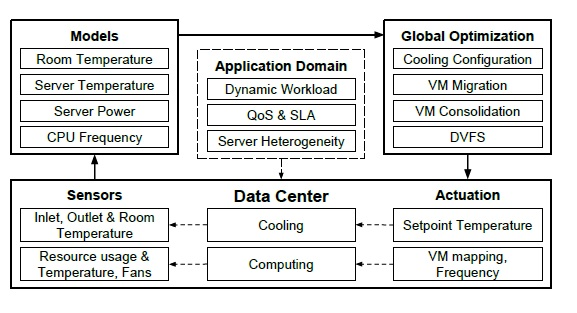
\includegraphics[width=100mm, height=49mm]{imagenes/capitulo1/1_2Esquema}
   \caption{Esquema del sistema de optimizaci'on. Fuente:\cite{Esquema}}
   \label{fig1_2:esq}
\end{figure}
	
	La soluci'on expuesta por \textit{GreenLSI} se basa en un sistema de monitorizaci'on y actuaci'on del CPD. Este sistema consta de una red de sensores distribuidos por el CPD que recoge datos de variables relacionadas con el consumo del CPD, tanto del entorno (temperatura, humedad, presi'on...) como de los equipos (frecuencia de la CPU, temperatura del equipo...). Por otro lado, se han elaborado una serie de modelos \cite{Modelos} que permiten estimar el valor de ciertos par'ametros relacionados con el consumo (temperatura de la sala, temperatura de los servidores, potencia de los servidores...).

	Con la informaci'on proporcionada por los sensores y utilizando los modelos de estimación, se realizan una serie de predicciones sobre el estado del CPD. Después, con las predicciones obtenidas, se realizan distintas optimizaciones tanto a nivel hardware como software, con el objetivo de que el CPD tenga un consumo 'optimo en ese estado. Por 'ultimo, se aplican esas optimizaciones realizando diferentes acciones sobre los elementos que conforman el CPD, ya sean los equipos IT o el sistema de refrigeraci'on. 

	En la figura \ref{fig1_2:esq} puede verse que una de las optimizaciones realizadas es la configuración de la refrigeración o \textit{cooling configuration}. Esta optimización consiste en ajustar la temperatura de la sala en base al estado del CPD y evitar el problema de sobreenfriamento de los equipos, con el objetivo de lograr un ahorro energético en el consumo global. Para ello, se irá modificando la temperatura de funcionamiento del sistema de refrigeración o \textit{setpoint}. Este trabajo se centrará en aplicar dicha optimación.

\section{Objetivos y fases del trabajo}\label{sec:obj}

	El propósito de este trabajo es diseñar un sistema de actuación que permita controlar la temperatura de la sala y fijarla en todo momento al valor proporcionado por el sistema de optimización energética. El sistema irá modificando el \textit{setpoint} del sistema refrigeración para lograr que la sala alcance la temperatura óptima. Para ello, el sistema de actuación debe tener las siguientes características:

	\begin{enumerate}
	\item\textbf{Autonomía:} el actuador tiene que llevar a cabo las acciones necesarias para fijar la temperatura de la sala sin intervención humana.
	\item\textbf{Dinámico:} el actuador debe responder a los cambios que se produzcan en la temperatura de optimización. Dicha respuesta debe hacerse a la mayor brevedad posible y teniendo en cuenta las limitaciones físicas que pudiera haber.
	\item\textbf{Estabilidad:} el actuador debe funcionar de una forma correcta, segura y sin comportamientos que puedan afectar al correcto funcionamiento del CPD.
	\item\textbf{No invasivo:} el funcionamiento del actuador no debe influir en el comportamiento normal de cada uno de los elementos del CPD.
	\item\textbf{Adaptable:} el actuador debe poder configurarse para que pueda ser usado en diferentes centros de datos. Dicha configuración tiene que ser sencilla y que implique el menor número de cambios posibles.
	\end{enumerate}

	En cuanto a las fases del trabajo, primero se exponen en el capítulo \ref{cap:estadoarte} los principales sistemas de control usados en la industria para controlar la temperatura. Después, en el capítulo \ref{cap:bancopruebas} se caracteriza el banco de pruebas usado para probar el actuador. A continuación, en los capítulos \ref{cap:dise'no} y \ref{cap:implementacion} se detallan todas las cuestiones relacionadas con el diseño y la implementación del actuador, respectivamente. Luego, en el capítulo \ref{cap:test} se muestran los experimentos realizados y se analizan los resultados obtenidos. Por último, en el capítulo \ref{cap:conclusiones}, se exponen las principales conclusiones de este trabajo y cuáles son sus principales líneas futuras.

	 \chapter{Estado del arte}\label{cap:estadoarte}

	El objetivo de este capítulo es dar una visión general de los sistemas o acciones de control que actualmente son utilizados en la industria para el control de magnitudes físicas, concretamente para controlar la temperatura. En este TFG el sistema de control es una pieza fundamental, ya que es el encargado de generar la señal de control que se aplica en todo momento al sistema de refrigeración para que la sala alcance la temperatura deseada.

	Primero se va a explicar el concepto de sistema de control y sus configuraciones más importantes. Después, se van a exponer las principales acciones de control usadas en la industria para realizar el control de la temperatura. Por último, se expone la situación actual en cuanto al control automático de la temperatura en los centros de datos.

\section{Sistema de control}

	Un sistema de control puede definirse como un conjunto de dispositivos encargados de administrar, dirigir o regular el comportamiento de otro sistema, y así obtener los resultados deseados. Si enfocamos la definición a este trabajo, la variable a controlar es la temperatura de la sala y esto se consigue controlando el comportamiento del sistema de refrigeración, es decir, su temperatura de funcionamiento o \textit{setpoint}. 

	Abstrayéndose de la aplicación concreta, un sistema de control sencillo básicamente posee una entrada de referencia y una salida o variable controlada. La entrada de referencia representa el valor que se desea que tenga la variable controlada y la función del sistema de control es conseguir que la variable controlada alcance ese valor. Dependiendo de si el sistema de control usa o no la entrada de referencia, podemos distiguir 2 tipos de configuración \cite{control1}:

	\textbf{Configuración en lazo abierto:} la variable controlada no es comparada con la entrada de referencia. Por lo tanto, cada valor de la entrada de referencia corresponde a una condición de operación fija. Esta configuración se usa principalmente en sistemas donde no hay perturbaciones y se conoce la relación entre la entrada y la salida. El motivo es que estos sistemas son fáciles de construir y mantener pero son más sensibles a las perturbaciones externas y la precisión de la salida depende de la calibración de los componentes, por lo que es complicado lograr que sean exactos. En la figura \ref{fig2_1:esquemacontrol} puede verse un esquema de esta configuración.

\begin{figure}[htbp]
	\centering
	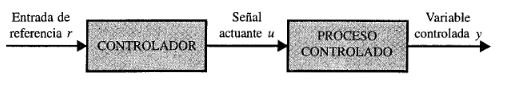
\includegraphics[width=120mm, height=20mm]{imagenes/capitulo2/2_1_1LazoAbierto}
   	\caption{Sistema de control en lazo abierto. Fuente: \textit{Benjamin C. Kuo}\cite{control2}}
   	\label{fig2_1:esquemacontrol}
\end{figure}

	\textbf{Configuración en lazo cerrado:} la variable controlada es medida y comparada con la entrada de referencia, generando una señal de error. Dicha señal es utilizada por el controlador para generar la señal de control y lograr que la variable controlada alcance el valor de la entrada. Los sistemas que usan esta configuración son más inmunes frente a las perturbaciones externas y más económicos en el sentido de que puede utilizar componentes más baratos y menos precisos para conseguir el ajuste deseado. Sin embargo, tienen mayores problemas de estabilidad porque el lazo de realimentación puede convertir un sistema estable en uno inestable. En la figura \ref{fig2_2:esquemacontrol} puede verse un esquema de esta configuración.

\begin{figure}[htbp]
	\centering
	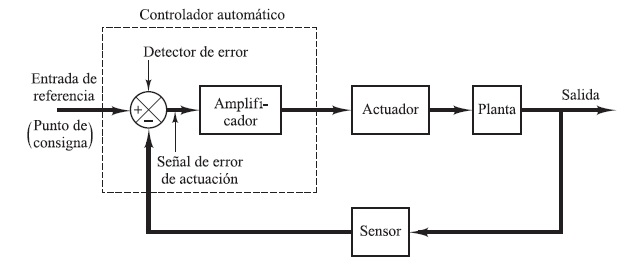
\includegraphics[width=110mm, height=40mm]{imagenes/capitulo2/2_1_2LazoCerrado}
   	\caption{Sistema de control en lazo cerrado. Fuente: \textit{Katsuhiko Ogata} \cite{control1}}
   	\label{fig2_2:esquemacontrol}
\end{figure}

	Hay que recalcar que los sistemas de control pueden tener múltiples entradas y múltiples salidas. Sin embargo, estas cuestiones no son tratadas en este TFG debido a que el control se realiza sobre una única variable.

\section{Tipos de controladores}

	En este apartado se explican los principales controladores utilizados por la industria para el control de la temperatura. Consultando algunos fabricantes de controladores como Omron \cite{fabricante1}, Omega \cite{fabricante2}, Coulton \cite{fabricante3} e Imopc\cite{fabricante4}, se puede deducir que los controladores más utilizados son:

\begin{itemize}
	\item{Controlador de 2 posiciones}
	\item{Controlador Proporcional (P)}
	\item{Controlador Proporcional-Integral-Derivativo (PID)}
\end{itemize}

	Para entender mejor su funcionamiento, también se van a explicar otros tipos de controladores  definidos en la teoría de control \cite{control1} \cite{control2} \cite{control3} y que también son usados en la industria. Estos controladores son:

\begin{itemize}
	\item{Controlador integral (I)}
	\item{Controlador Derivativo (D)}
	\item{Controlador Proporcional-Integral (PI)}
	\item{Controlador Proporcional-Derivativo (PD)}
\end{itemize}

\subsection{Controlador de 2 posiciones}\label{sec:On-Off}
	También es conocido como controlador \textit{On-Off} o \textit{todo-nada}. Es un controlador sencillo y barato, por lo que su uso está extendido tanto en sistemas de control industriales como domésticos. 

	La señal de control $m(t)$ conmuta entre 2 valores posibles, en función de la señal de error $e(t)$. En la figura \ref{fig2_1:histeresis} se muestra el esquema de funcionamiento.

\begin{figure}[htbp]
\centering
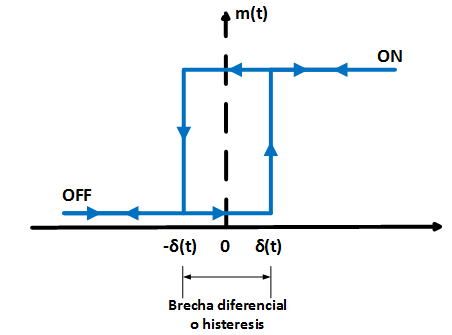
\includegraphics[width=85mm,height=50mm]{imagenes/capitulo2/2_1_On-Off}
\caption {Esquema de funcionamiento del controlador \textit{On-Off} }
\label{fig2_1:histeresis}
\end{figure}

	En dicha figura puede verse que la conmutación no se realiza en 0 sino en los extremos de un intervalo denominado \textit{brecha diferencial o histéresis}. Este mecanismo permite evitar daños en los componentes de la planta cuando la conmutación entre los 2 estados se realiza de manera muy rápida. La señal de control no conmuta hasta que la señal de error supera una cierta cantidad $\delta(t)$, tanto si el error es positivo ($e(t) > \delta(t)$) como si es negativo ($e(t) < -\delta(t)$). En ocasiones puede fijarse ese intervalo a 0, siempre y cuando la conmutación no sea muy rápida y se garantice el correcto funcionamento de la planta.

	El funcionamiento del controlador es el siguiente: supongamos que la señal de control está en OFF y el error es negativo. Cuando $e(t) > \delta(t)$, la señal de control conmuta al estado ON. Este estado habitualmente se traduce en una acción que hace que la planta a controlar se encienda y funcione (enceder un motor, abrir una válvula...). 

	Supongamos ahora que la señal de control está en ON y el error es positivo. Si se cumple que $e(t) < -\delta(t)$, la señal de control conmuta al estado OFF. Este estado habitualmente se traduce en una acción que hace que la planta a controlar se apague o deja de funcionar (apagar un motor, cerrar una válvula...).

\begin{figure}[htbp]
\centering
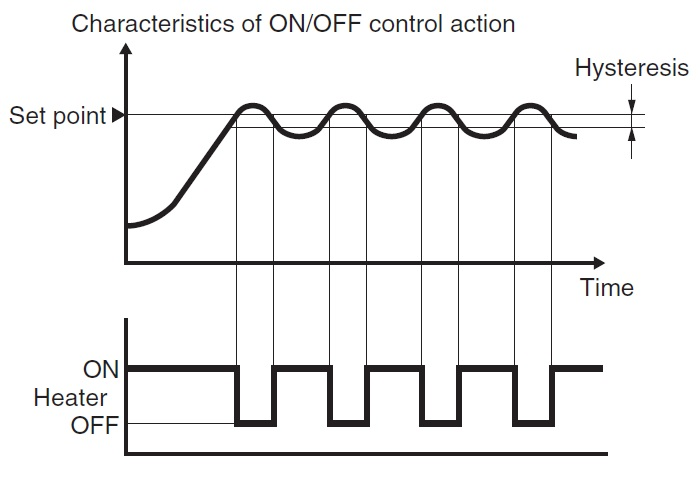
\includegraphics[width=85mm,height=45mm]{imagenes/capitulo2/2_2_On-Off}
\caption {Respuesta de un sistema con un controlador \textit{On-Off}. Fuente: Omron \cite{fabricante1}}
\label{fig2_2:on-off}
\end{figure}

	El funcionamiento del controlador es sencillo aunque presenta limitaciones en cuanto a que sólo puede usarse para aquellos sistemas que puedan ser controlados mediante 2 estados de funcionamiento.

\subsection{Controlador proporcional (P)}

	Su acción se basa en multiplicar la señal de error por una constante denominada \textit{constante proporcional} $K_{p}$. Su expresión matemática es la siguiente:
\begin{equation}\label{ecuacion2_1}
\normalsize m_{P}(t) =K_{p}e(t)
\end{equation}

	El controlador amplifica la señal de error para conseguir que la señal medida siga a la señal de referencia. Sin embargo, analizando la ecuación, se ve que no se consigue eliminar el error estacionario ya que si el error fuese nulo, la señal de control también lo sería. 

	Este controlador puede ajustarse a través de la constante $K_{p}$ o mediante el concepto de la \textbf{banda proporcional}, que se define como la cantidad que tiene que cambiar la variable controlada para lograr un cambio del 100\% en la acción de control. Su expresión matemática es  $BP\%=\frac{100}{K_{p}}$ y es un concepto similar a la ganancia proporcional. En la figura \ref{fig2_3_1:proporcional} se muestra una gráfica que representa el comportamiento de esta acción.

\begin{figure}[htbp]
\centering
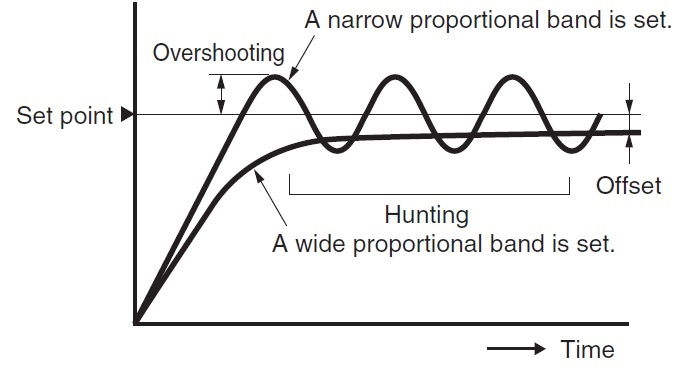
\includegraphics[width=90mm,height=45mm]{imagenes/capitulo2/2_3_1_Proporcional}
\caption {Respuesta de un sistema con un controlador P. Fuente: Omron \cite{fabricante1}}
\label{fig2_3_1:proporcional}
\end{figure}

	En dicha gráfica puede verse que si la banda proporcional es amplia (equivale a una $K_{p}$ pequeña), la respuesta de la planta se aproxima al valor de referencia pero tiene un ligero offset, mientras que si la banda es reducida (equivale a una $K_{p}$ grande), la respuesta presenta oscilaciones entorno al valor de referencia.

\subsection{Controlador Integral (I)}

	Su acción se basa en integrar la señal de error y multiplicarla por una constante denominada \textit{constante integral} $K_{i}$. Su expresión matemática es la siguiente:
\begin{equation}\label{ecuacion2_2}
\normalsize m_{I}(t) = K_{i}\int _0^t e(t) dt
\end{equation}
	
	El controlador genera una señal que es función de la "historia"~ de la señal de error, lo que permite conseguir una señal de control no nula aunque la señal de error sí lo sea. Este controlador consigue eliminar el error estacionario aunque empeora la estabilidad del sistema, aumentando el sobreimpulso de la respuesta transitoria e incluso puede hacer que el sistema se vuelva inestable.  No suele utilizarse sólo sino que se combina con otras acciones de control, por ejemplo, con un controlador proporcional.

\subsection{Controlador Proporcional Integral (PI)}

	Este controlador se basa en una combinación de la acción proporcional y la acción integral. Su expresión matemática es la siguiente:
\begin{equation}\label{ecuacion2_3}
\normalsize m_{PI}(t) =K_{p}e(t) + K_{i}\int _0^t e(t) dt = K_{p}\left( e(t) + \frac{1}{T_{i}} \int _0^t e(t) dt\right)
\end{equation}

	Ajustando los parámetros $K_{p}$ y $K_{i}$ se consigue ajustar la respuesta a los requisitos deseados. El ajuste de la acción integral puede realizarse mediante $K_{i}$  o usando un parámetro denominado \textit{tiempo integral} $T_{i}$, que se define como $T_{i}=\frac{K_{p}}{K_{i}}$.

	En la figura \ref{fig2_3_2:PI} se muestra la respuesta de una planta con este controlador. En dicha figura se observa como la acción integral consigue eliminar el error estacionario y que la respuesta se aproxime al valor deseado. Es necesario ajustar correctamente los valores $K_{p}$ y $K_{i}$, ya que puede ocurrir que la señal tenga un mayor sobreimpulso o que sea demasiado lenta y tarde más tiempo en alcanzar el estado estacionario.

\begin{figure}[htbp]
\centering
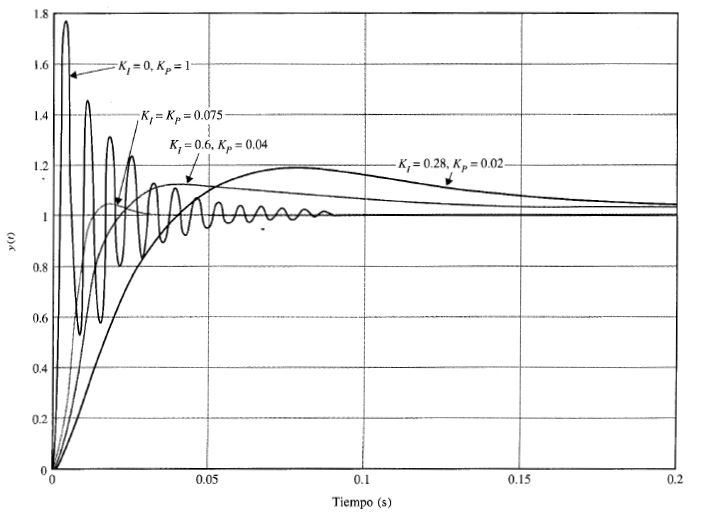
\includegraphics[width=100mm,height=55mm]{imagenes/capitulo2/2_3_2_PI}
\caption {Respuesta de un sistema con una acción PI. Fuente: \textit{Benjamin C. Kuo} \cite{control2}}
\label{fig2_3_2:PI}
\end{figure}

\subsection{Controlador Derivativavo (D)}

	Su acción se basa en derivar la señal de error y multiplicarla por una constante denominada \textit{constante derivativa} $K_{d}$. Su expresión matemática es la siguiente:
\begin{equation}\label{ecuacion2_4}
\normalsize m_{D}(t) = K_{d}\frac{de(t)}{dt}
\end{equation}

	Esta acción añade sensibilidad al sistema y permite corregir el error antes de que se vuelva excesivo. Provoca un aumento en la estabilidad relativa que se traduce en un menor sobreimpulso y una respuesta con un menor tiempo de subida y de establecimiento. Sin embargo, no puede utilizarse sólo porque no es capaz de eliminar el error estacionario para una señal constante.  Suele combinarse con otras acciones de control, por ejemplo, con un controlador proporcional.

\subsection{Controlador Proporcional Derivativo (PD)}

	Este controlador se basa en la combinación de la acción proporcional y la acción derivativa. Su expresión matemática es la siguiente:
\begin{equation}\label{ecuacion2_5}
\normalsize m_{PD}(t) =K_{p}e(t) + K_{d}\frac{de(t)}{dt} = K_{p}\left( e(t) + T_{d}\frac{de(t)}{dt}\right)
\end{equation}

	Ajustando los parámetros $K_{p}$ y $K_{d}$ se consigue ajustar la respuesta a los requisitos deseados. El ajuste de la acción derivativa puede hacerse mediante $K_{d}$ o con un parámetro denominado \textit{tiempo derivativo} $T_{d}$, que se define como $T_{d}=\frac{K_{d}}{K_{p}}$.

\begin{figure}[htbp]
\centering
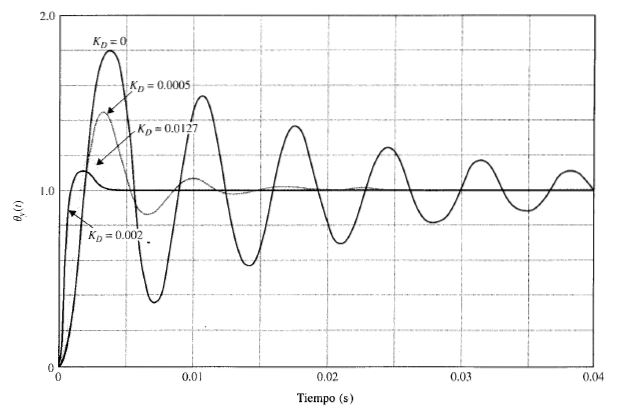
\includegraphics[width=100mm,height=55mm]{imagenes/capitulo2/2_3_3_PD}
\caption {Respuesta de un sistema con una acción PD. Fuente: \textit{Benjamin C. Kuo}\cite{control2}}
\label{fig2_3_3:PD}
\end{figure}
	
	En la figura \ref{fig2_3_3:PD} se muestra la respuesta de una planta con este controlador. En dicha figura se observa que a medida que aumenta la acción derivativa, la respuesta tiene un menor sobreimpulso, es más rápida y tiene un menor tiempo de establecimiento. 

\subsection{Controlador PID}
	Combina las ventajas de las 3 acciones . Su expresión matemática es:
\begin{equation}\label{ecuacion2_6}
\normalsize m(t) =K_{p}e(t) + K_{i}\int _0^t e(t) dt + K_{d}\frac{de(t)}{dt} =  K_{p}\left( e(t) + \frac{1}{T_{i}} \int _0^t e(t) dt + T_{d}\frac{de(t)}{dt}\right)
\end{equation}

	En la figura \ref{fig2_4:PID} se compara la respuesta de una planta usando un controlador PID frente a un controlador PI y un controlador PD. Ajustando los parámetros adecuadamente, se consiguen los resultados deseados. Este controlador es ampliamente usado en la industria debido a que puede adaptarse a un amplio rango de valores de funcionamiento y a que posee un planteamiento sencillo. 

\begin{figure}[htbp]
\centering
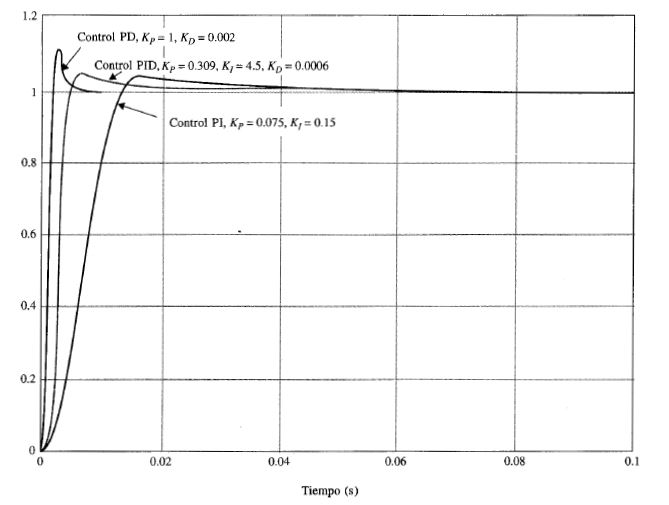
\includegraphics[width=90mm,height=55mm]{imagenes/capitulo2/2_4_PID}
\caption {Respuesta de un sistema usando un PID. Fuente: \textit{Benjamin C. Kuo} \cite{control2}}
\label{fig2_4:PID}
\end{figure}

	Este controladores posee diferentes representaciones, dependiendo de las necesidades. En la figura \ref{fig2_5:PID} se muestran algunas de ellas.  El 1º esquema es la representación paralela o ideal y se caracteriza en que cada una de las acciones no se influyen mutuamente. Su expresión matemática es la primera parte de la ecuación \ref{ecuacion2_6}.

	 El esquema central es la representación estándar o no interactiva y se basa en que la acción proporcional influye en el resto de acciones pero la acción integral y derivativa no se influyen entre sí. Su expresión matemática es la segunda parte de la ecuación \ref{ecuacion2_6}. Por último, la figura de la derecha es la representación serie o interactuante y se caracteriza porque la acción integral influye en la derivativa o vicerversa.

\begin{figure}[htbp]
\centering
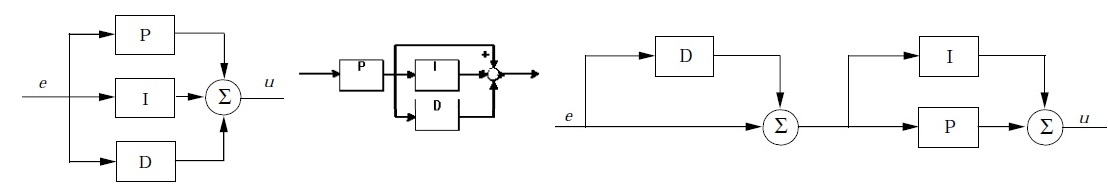
\includegraphics[width=110mm,height=30mm]{imagenes/capitulo2/2_5_PID}
\caption {Esquemas de representación de un PID. Fuente: \textit{Katsuhiko Ogata} \cite{control3}}
\label{fig2_5:PID}
\end{figure}

	Este controlador tiene un funcionamiento lineal pero en muchas ocasiones pueden aparecer efectos no lineales. Una no linealidad típica es el efecto windup. El actuador posee un rango de funcionamiento limitado y si el sistema de control tiene un amplio rango de operación, puede ocurrir que la señal de control alcance el límite del actuador.

	Cuando esto sucede, el lazo de realimentación se rompe porque el actuador se satura y deja de seguir a la señal de control. Sin embargo, el error se sigue acumulando y la señal de control sigue aumentando. Cuando la señal de error cambia de signo, la señal de control empieza a reducirse pero requiere de un gran tiempo para volver a entrar en la región lineal. Esto provoca grandes transitorios en la respuesta de la planta. En la figura \ref{fig2_6:windup} se representa este efecto.  

\begin{figure}[htbp]
\centering
\includegraphics[width=110mm,height=25mm]{imagenes/capitulo2/2_6_Windup}
\caption {Representación del efecto windup. Fuente: \textit{Katsuhiko Ogata} \cite{control3}}
\label{fig2_6:windup}
\end{figure}

	Para solucionarlo, existen varios métodos como limitar el valor de referencia para que la señal de control no alcance los límites del actuador, la integración condicional que se basa en habilitar la acción integral si se cumplen determinadas condiciones o la técnica del recálculo y seguimiento que recalcula la integral cuando el actuador se satura y consigue que la señal de control se aproxime al límite del actuador \cite{control3}. 

\section{Control de temperatura}

	En este apartado se pretende exponer cómo se realiza el control de la temperatura en un centro de datos, es decir, como se ajusta el valor de referencia según la situación del CPD.

	En la actualidad, existen diferentes herramientas de control y gestión de los centros de datos, como Data Center Infraestructure Management (DCIM) o Supervisory Control And Data Adquisition (SCADA). 

	El sistema SCADA supervisa y controla las operaciones a través de sensores que están colocados en diferentes lugares y que son monitorizados desde una unidad centralizada. Las funciones incluyen gestión de alarmas, diagnóstico, mantenimiento, interfaces gráficas que muestran la situación actual del CPD, entre otros. 

	El sistema DCIM está formado por un sistema software, hardware y sensores que permiten gestionar, supervisar y planificar la capacidad de la infraestructura crítica de un CPD. El sistema maneja los datos proporcionados por los sensores y con ellos puede gestionar tanto los servidores como el resto de equipos. Dispone de una plataforma de gestión y monitorización para visualizar el estado del CPD en tiempo real.

	Sin embargo, estos sistemas son complejos de manejar y requieren de algún tipo de intervención humana, incluyendo el caso de  la temperatura. Estos sistemas monitorizan y controlan la temperatura pero se necesita un operario para realizar los cambios.

	Por tanto, el sistema de actuación diseñado en este trabajo debe ser capaz de proporcionar al controlador el dato óptimo de temperatura de una forma automática y sin ningún tipo de acción humana.

	\chapter{Banco de pruebas}\label{cap:bancopruebas}

	En este capítulo se describe el banco de pruebas en el que se va a verificar el funcionamiento del actuador. También se detallan algunas características del banco que son importantes para la etapa de diseño.

	El banco de pruebas elegido es la sala B039 del Departamento de Ingeniería Electrónica. En esta sala se guardan gran parte de los servidores que almacenan la informaci'on del departamento, por lo que se trata de un entorno real y adecuado para probar el actuador. Además, se encuentra monitorizado y está implementado una parte del sistema de monitorización explicado en el apartado \ref{sec:enfoque}. En la figura \ref{fig3_1:sala} se muestra una imagen de dicha sala.

En esta sala existen 2 sistemas de refrigeraci'on. Sus características son las siguientes:

\begin{itemize}
	\item\textbf{Sistema de refrigeraci'on del edificio:} su principal objetivo es mantener una temperatura de confort en cada una de las salas del edificio. Sin embargo, este sistema no es suficiente para evacuar el calor generado por los equipos, debido a que s'olo funciona durante los meses de verano. Además, no existe ningún mecanismo que permita controlar el sistema para que se pueda fijar la temperatura de esta sala según sus necesidades y de manera independiente al resto de salas del edificio. Por tanto, este sistema es descartado para el control de la temperatura.

	\item\textbf{Unidad de refrigeraci'on comercial:} su objetivo es la evacuaci'on del calor generado por los equipos de la sala. Este sistema funciona durante todo el a'no y permite configurar el \textit{setpoint}. Por tanto, el control de la temperatura se va a realizar utilizando este sistema.
\end{itemize}

\begin{figure}[h]
\centering
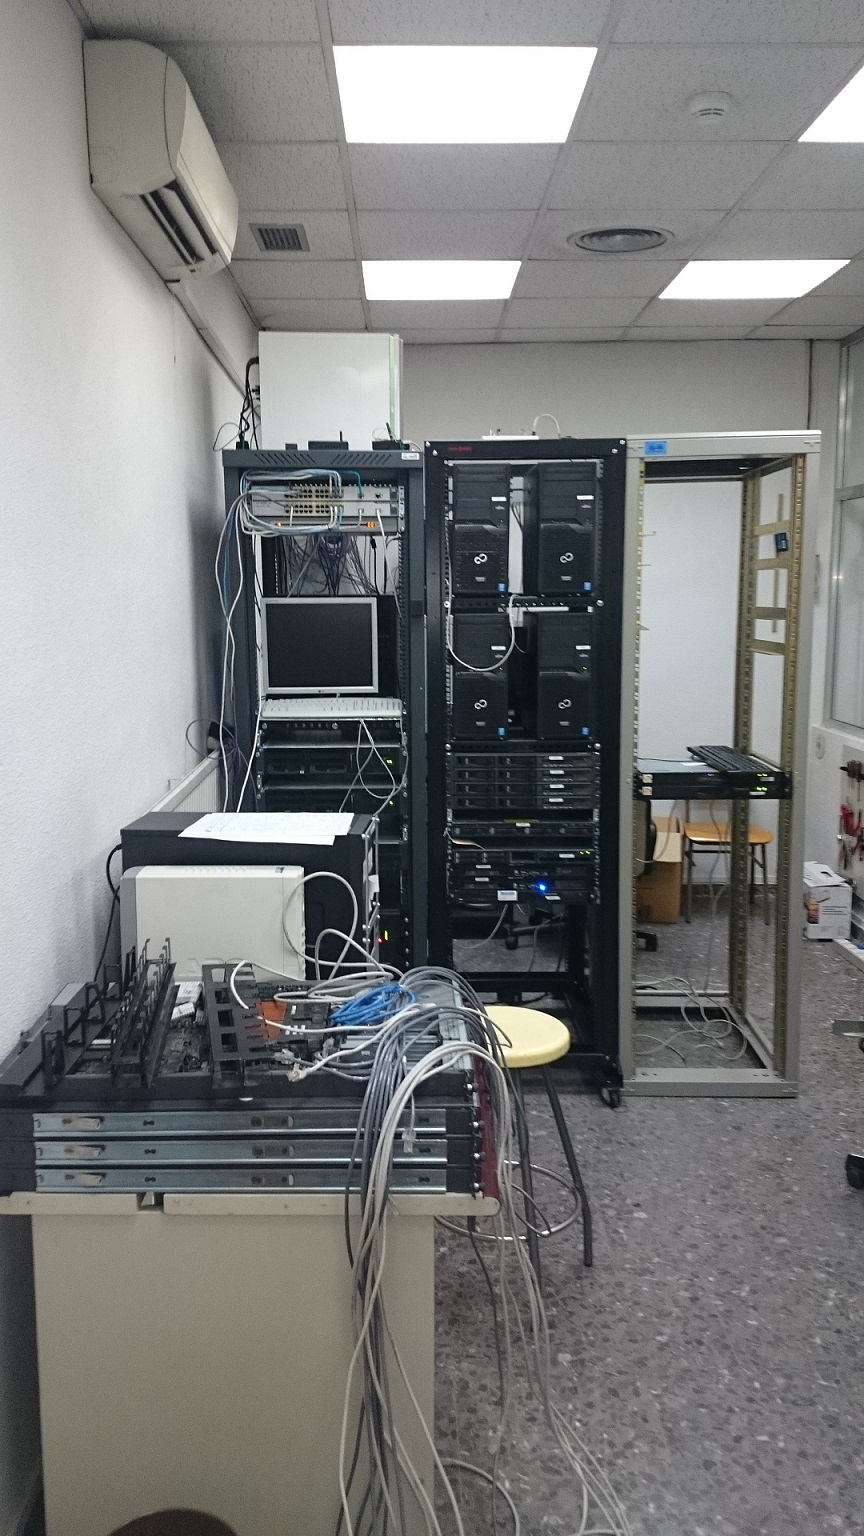
\includegraphics[width=0.55\textwidth,height=105mm]{imagenes/capitulo3/bancoPruebas2}
\caption {Fotograf'ia de la sala B039}
\label{fig3_1:sala}
\end{figure}

	El control del \textit{setpoint} se realiza de forma manual y a través de un mando a distancia. Este mando dispone de varias teclas que permiten configurar el modo de funcionamiento. Al pulsar alguna de estas teclas se envía una orden al sistema de refrigeración para que modifique su estado de funcionamiento.

	Cada una de las órdenes o modos de funcionamiento es representada a través de un comando. El comando está formado por una secuencia de bits con un determinado protocolo o formato que es interpretado por el receptor situado en la unidad de refrigeración. El receptor decodifica la secuencia recibida y en base a ello, modifica el funcionamiento del sistema de refrigeración.

	Cada comando es enviado al receptor mediante una señal de infrarrojos. Dicha señal está modulada a una frecuencia de 38 KHz, que es la frecuencia de portadora fijada por el fabricante para la comunicación a través del mando a distancia. El sistema posee un rango de funcionamiento que va de 18{$^\circ$}C a 32{$^\circ$}C, con saltos de 1{$^\circ$}C entre 2 temperaturas consecutivas. 

	Por tanto, la comunicación del sistema de actuación con la unidad de refrigeración deberá realizarse mediante un sistema de infrarrojos que emule el comportamiento del mando a distancia y que lo haga de manera automática. Además, deberá tener en cuenta las cuestiones mencionadas sobre el rango de funcionamiento y la modulación.







	\chapter{Dise'no}\label{cap:dise'no}

	En este capítulo se expone de manera detallada el dise'no del sistema de actuaci'on y se analiza cada uno de los subsistemas que lo componen. El diseño se ha hecho teniendo en cuenta los requisitos indicados en el apartado \ref{sec:obj} del capítulo \ref{cap:intro}. 

\section{Descripci'on del sistema completo}\label{sec:arq_actuador}

	La arquitectura elegida se basa en un sistema de control en lazo cerrado, ya que hace al sistema m'as inmune frente a las perturbaciones y logra unos mejores ajustes. No se ha escogido la configuración en lazo abierto porque requiere de unos ajustes más precisos y es más sensible a las perturbaciones. Además, la temperatura de la sala depende de factores como el aislamiento de la sala, la temperatura exterior, el calor generado por los equipos, etc, cuyo impacto en la respuesta global es difícil de caracterizar con exactitud. En la figura \ref{4_1:diag_completo} se muestra un esquema de la arquitectura. 

\begin{figure}[htbp]
  \centering
  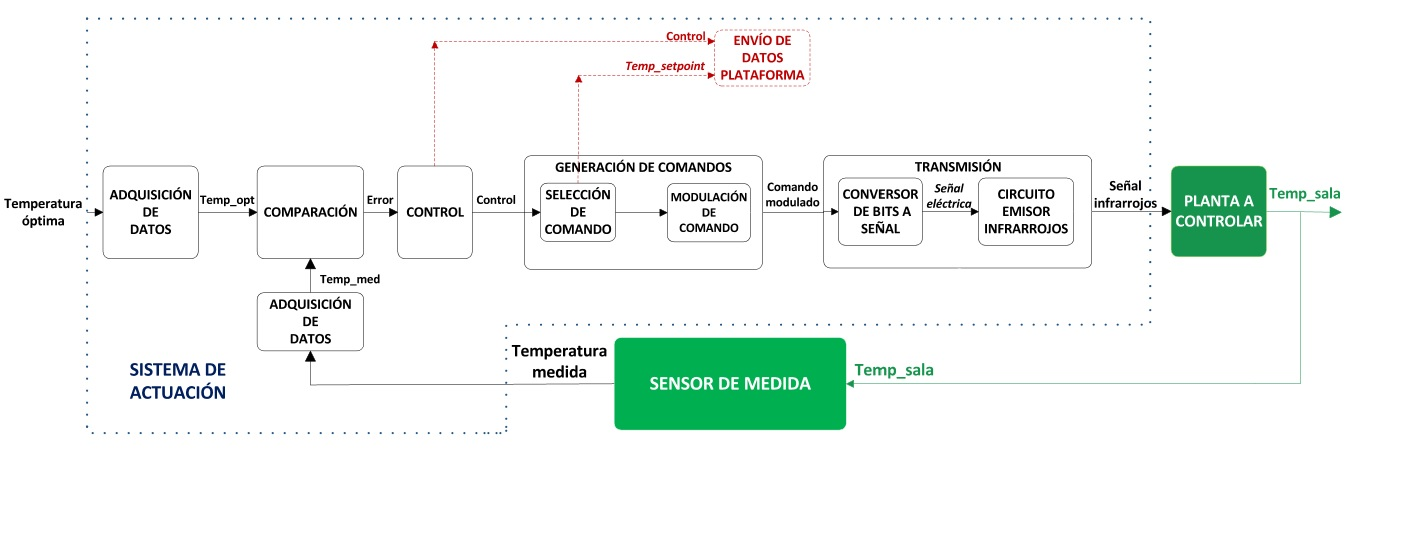
\includegraphics[width=95mm, height=220mm]{imagenes/capitulo4/4_1Diagrama_Completo}
   \caption{Diagrama del sistema completo}
   \label{4_1:diag_completo}
\end{figure}

	El sistema de actuaci'on tiene 2 entradas: la temperatura a la que debe estar la sala o \textit{temperatura 'optima}, proporcionada por el sistema de optimización y la temperatura a la que se encuentra la sala o \textit{temperatura medida},  proporcionada por el sensor. El sistema tiene una única salida que es el \textit{setpoint} del aire acondicionado. El sistema est'a formado por los siguiente bloques:
\begin{itemize}
    	\item Bloque de adquisici'on de datos.
    	\item Bloque de comparaci'on.
    	\item Bloque de control.
    	\item Bloque de generaci'on del comando.
    	\item Bloque de transimisi'on.
\end{itemize}

	En la figura \ref{4_1:diag_completo} tambi'en se incluyen la planta a controlar y el sensor de medida. Estos componentes son fundamentales para explicar el funcionamiento del actuador pero no forman parte de él, por lo que no son considerados en la etapa de dise'no. 

	Tambi'en existe un bloque de env'io de datos que se utiliza para mandar datos a la plataforma de monitorización y poder visualizar y evaluar el correcto funcionamiento del actuador. Este bloque se incluye en el dise'no, aunque no es fundamental para el funcionamiento del actuador.

	En los siguientes apartados se hace una descripci'on detallada de cada uno de los bloques del actuador.

\section{Bloque de adquisici'on de datos}\label{sec:adquisicion}

	Es la primera etapa del sistema de actuaci'on. El dato de \textit{temperatura 'optima} y el dato de \textit{temperatura medida} se encuentran almacenados en una plataforma y con un determinado formato. Hay que tener en cuenta el tipo de plataforma y el formato utilizado, ya que ambos varían seg'un el CPD e incluso puede darse el caso de que ambos datos est'en almacenados en plataformas diferentes y con distintos formatos. Tambi'en hay que considerar que el dato puede estar almacenado con un formato que no permite al actuador utilizarlo directamente y necesita ser procesado.

	El actuador va a disponer de 2 bloques de adquisici'on, uno para cada dato. Cada bloque tendr'a como entrada el dato de temperatura almacenado en la plataforma y como salida ese mismo dato procesado para que el actuador pueda utilizarlo. En la figura \ref{4_2:diag_adquisicion} se muestra un esquema de cada uno de estos bloques.	

\begin{figure}[htbp]
  \centering
  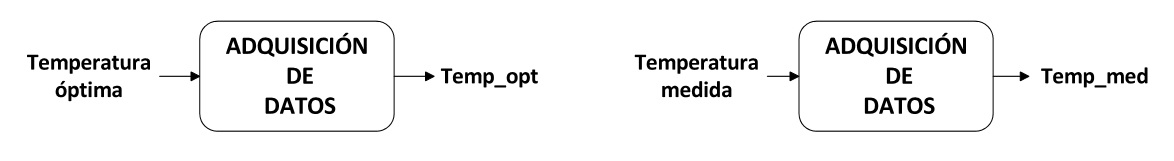
\includegraphics[width=142mm,height=20mm]{imagenes/capitulo4/4_2Bloque_Adquisicion}
   \caption{Esquema del bloque de adquisici'on de datos}
   \label{4_2:diag_adquisicion}
\end{figure}

	Para este trabajo se va a usar \textit{Graphite} como plataforma de almacenamiento de datos debido a que los sensores de la sala B039 env'ian los datos a un servidor que utiliza dicha plataforma. Según su documentación \cite{Graphite1}, \textit{Graphite} almacena series de datos junto con su marca temporal o \textit{timestamp}. Adem'as, proporciona una aplicaci'on web a trav'es de la cual se pueden visualizar los datos de forma gr'afica o se pueden exportar en diferentes formatos. En la figura \ref{4_3:interfaz_graphite} se muestra una imagen de la interfaz gr'afica de \textit{Graphite}.

\begin{figure}[htbp]
  \centering
  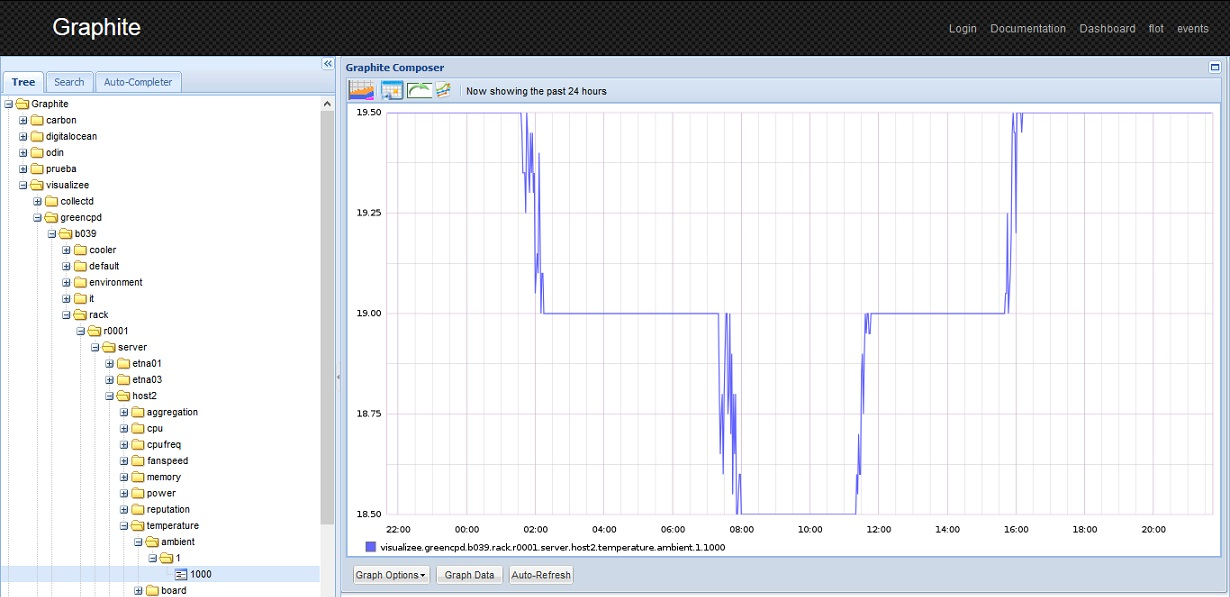
\includegraphics[width=140mm, height=75mm]{imagenes/capitulo4/4_3Interfaz_Graphite}
   \caption{Interfaz gr'afica de \textit{Graphite}}
   \label{4_3:interfaz_graphite}
\end{figure}

	\textit{Graphite} permite exportar los datos que tiene almacenados, en diferentes formatos. De entre todos ellos, se ha decidido utilizar JSON. El motivo es que tiene un esquema de representación fácil de entender y el procesamiento del dato es más fácil de hacer en este formato que en el resto de formatos existentes. A continuación se muestra un ejemplo de un dato que ha sido exportado de \textit{Graphite} en formato JSON:

\begin{verbatim}
   [{"target":visualizee.greencpd.rack.b039.cooler.temperature.supply.
   setpoint.2, "datapoints": [[18.0, 1496395200], [18.0, 1496395210], 
   [19.0, 1496395220], [21.0, 1496395230], [23.0, 1496395240], 
   [22.0, 1496395250]]}]
\end{verbatim}

	El objeto JSON posee 2 campos: \textbf{target} y \textbf{datapoints}. El campo \textbf{target} almacena una cadena de caracteres con la ruta en la que se encuentra el dato que se quiere exportar. El campo \textbf{datapoints} es un array de N-duplas donde cada dupla contiene el valor de la temperatura junto con el instante de medida o \textit{timestamp}. El valor de la temperatura es un n'umero real con una precisi'on de cent'esimas y el \textit{timestamp} es un entero que expresa el tiempo en formato epoch.

	Los datos almacenados en \textit{Graphite} se pueden exportar realizando una petici'on http. A continuaci'on se muestra un ejemplo del formato de una url usada para exportar un dato de la plataforma.

\begin{verbatim}
http://visualizee.die.upm.es:8000/render?format=json&target=visualizee.
.greencpd.b039.rack.r0001.server.host2.temperature.ambient.1.1000
&from=-1min&until=-4min
\end{verbatim}

	 Según la documentación \cite{Graphite1}, la url contiene 4 par'ametros que son configurados para seleccionar el dato que se desea exportar, el formato en el que se obtienen los datos y el número de muestras que se van a exportar. Estos par'ametros son:

\begin{itemize}
\item \textbf{format:} contiene el formato en el que se desea extraer los datos.
\item \textbf{target:} contiene la ruta donde se encuentra el dato a exportar.
\item \textbf{from:} contiene el instante de inicio de la toma de muestras. Si no se especifica nada, se toma por defecto las 'ultimas 24 horas. 
\item \textbf{until:} contiene el instante final de la toma de muestras. Si no se especifica nada, se toma por defecto el instante actual.
\end{itemize}

	En cada petición es recomendable exportar varias muestras y no sólo la del instante de la iteración, ya que puede darse el caso de que el sistema de actuación haga la petición del dato de temperatura y el sensor todavía no lo haya medido o genere null. De este modo, se soluciona este problema y el error cometido es mínimo porque la temperatura es una variable que evoluciona lentamente y la variación que puede producirse entre muestras muy próximas es muy pequeña. En este trabajo, el sensor de banco de pruebas toma muestras cada 10 segundos, luego se van a exportar las muestras de \textit{temperatura óptima} y \textit{temperatura medida} tomadas en el último minuto para tener un cierto margen de seguridad.

	Por 'ulltimo, una vez exportado el dato de la plataforma y extraído del objeto JSON, éste se multiplica por un factor de conversi'on para convertirlo a un número entero que tenga la precisión necesaria para ser utilizado en las siguientes etapas. En este trabajo, el bloque de comparación y de control van manejar números enteros que representan a números reales con una precisión de milésimas. Por tanto, el factor de conversión es 1000. De este modo, se conserva la precisión del dato de temperatura y ya está preparado para ser usado en próximas etapas.

\section{Bloque de comparaci'on}\label{sec:comparacion}

Su función es calcular el error que hay entre la \textit{temperatura 'optima} y la \textit{temperatura medida}. En la figura \ref{4_4:diag_comparacion} se muestra un diagrama de este bloque. 

\begin{figure}[htbp]
  \centering
  \includegraphics[width=100mm, height=25mm]{imagenes/capitulo4/4_4_Bloque_Comparacion}
   \caption{Diagrama del bloque de comparaci'on}
   \label{4_4:diag_comparacion}
\end{figure}

	El bloque resta a la \textit{temperatura óptima} el valor de la \textit{temperatura medida}. El resultado de dicha operación es el valor de la señal de error. El error está expresado en las mismas unidades que las temperaturas.

\section{Bloque de control}\label{sec:control}

	Su función es generar la señal de control que se enviará al sistema de refrigeración para que la sala alcance la \textit{temperatura óptima}. Dicha señal es generada a partir de la señal de error y siguiendo un determinado algoritmo o pol'itica de control. En la figura \ref{4_5:diag_control} se muestra un esquema con las entradas y salidas del bloque.

\begin{figure}[htbp]
  \centering
  \includegraphics[width=100mm, height=22mm]{imagenes/capitulo4/4_5_Bloque_Control}
   \caption{Esquema del bloque de control}
   \label{4_5:diag_control}
\end{figure}

	De todos los controladores explicados en el capítulo \ref{cap:estadoarte}, se ha escogido el controlador PID, ya que es un controlador ampliamente usado en la industria, incluyendo procesos de control de la temperatura, con un planteamiento sencillo y con diferentes métodos de diseño y ajuste. Se ha decidido usar la representación ideal o paralela.

	El ajuste del controlador puede realizarse tanto en el dominio del tiempo como en la frecuencia \cite{PID}. Algunos de los métodos utilizados son: Ziegler-Nichols, diagrama de bode, criterio de Routh-Hurwitz, lugar de raíces, método de prueba y error... 

	Algunos de estos métodos permiten el ajuste de la planta sin necesidad de conocer su función de transferencia. Sin embargo, es recomendable obtener dicha función, para así facilitar el proceso de ajuste de los parámetros. Por otro lado, la expresi'on anterior está definida para un controlador en tiempo continuo. Sin embargo, el controlador se va a implementar en un sistema digital, luego es necesario discretizarlo. 

	Por tanto, el proceso de diseño del controlador consta de las siguientes fases: primero, se estima la función de transferencia que modela la planta a controlar. Después, se diseña el controlador PID y se ajustan sus parámetros usando alguno de los métodos anteriormente descritos. Por último, se discretiza el controlador PID diseñado. A continuación, se explican cada una de estas fases en los siguientes apartados.

\subsection{Caracterizaci'on de la planta}\label{subsec:caract_planta}

	En esta fase se va a estimar la función de transferencia que representa el comportamiento dinámico de la planta. La variable a controlar es la temperatura de la sala y dicho control se va a realizar a trav'es del sistema de refrigeraci'on de la sala. Por tanto, la planta a controlar está formada por el sistema de refrigeraci'on y la sala. 

	La planta puede ser caracterizada aplicando modelos f'isicos de los distintos componentes que componen la planta (ciclo de refrigeración + sala). Sin embargo, esto es poco viable porque hay par'ametros que son dif'iciles de caracterizar y medir. 

	Por este raz'on, se decide hacer la caracterizaci'on de la sala mediante la t'ecnica de identificaci'on de sistemas. Se van a realizar una serie de experimentos basados en excitar la planta con una se'nal de entrada específica (escalón, rampa...) y se miden los valores generados en la salida. Despu'es, se aplican m'etodos estad'isticos que permiten estimar una funci'on matem'atica que representa el comportamiento de la planta. 

	El experimento realizado en este trabajo se basa en aplicar una se'nal de entrada de tipo escal'on al sistema de refrigeraci'on y medir la temperatura de la sala. El valor inicial y el valor final de la señal escalón son el valor mínimo y máximo de funcionamiento del sistema de refrigeración (18{$^{\circ}$}C y 32{$^{\circ}$}C respectivamente). De este modo,se pretende abarcar todo el rango de  de funcionamiento del sistema de refrigeración y caracterizar mejor la planta. 

	Hay que tener en cuenta que aunque la temperatura máxima sea de 32{$^{\circ}$}C, la sala no puede alcanzar ese valor, ya que la temperatura máxima recomendada para el buen funcionamiento de la sala está entre (25{$^{\circ}$}C - 27{$^{\circ}$}C) y si se supera, podrían dañarse los equipos. Por tanto, el experimento se mantendrá hasta que la sala alcance ese valor recomendado. 

	Los valores de la salida son medidos cada 10 segundos, ya que es el periodo de muestreo del sensor. Podr'ia haberse elegido un periodo de muestreo superior, por ejemplo 1 min, ya que la evoluci'on de la temperatura es un proceso lento. Sin embargo, se opta por un periodo igual al periodo de muestreo del sensor y se evita tener que hacer un procesamiento adicional. Este experimento se repetirá varias veces para obtener un mayor n'umero de muestras.

	Una vez realizados todos los experimentos, se estima la funci'on transferencia de la planta, utilizando el programa de c'alculo matem'atico MATLAB. Se va a dise'nar un script con el que se obtiene los valores de la se'nal de entrada y de salida utilizadas en cada experimento. Después se estima la función de transferencia usando la funci'on de matlab \textit{tfest}. Esta funci'on toma como par'ametros los datos de entrada y de salida y el n'umero de polos y ceros del sistema. Para cada conjunto de datos se van a realizar todas las combinaciones posibles de polos y ceros hasta orden 3, ya que este tipo de sistemas suelen ser de 1{$^{\circ}$}o 2{$^{\circ}$} orden y no es recomendable usar sistemas cuyo orden es muy elevado debido al problema de sobreajuste u \textit{overfitting}. El objetivo es estimar una función que tenga un buen ajuste con cualquier conjunto de datos.

	Una vez se han obtenido todas las combinaciones, se escoge aquella que tenga un mejor coeficiente de ajuste. Este coeficiente de ajuste es proporcionado por la misma función \textit{tfest} y es calculado mediante el error cuadr'atico medio normalizado o NRMSE \textit{Normalized Root-Mean-Square Error}. 

	La función \textit{tfest} presenta el inconveniente de que sólo puede manejar un conjunto de datos a la vez, por lo que no se puede calcular una estimación basada en los conjuntos de datos de todos los experimentos. Para solucionar este problema, se calcula el coeficiente de ajuste que tiene cada funci'on de transferencia de cada experimento, con respecto a sus datos y a los datos de los otros experimentos y se calcula el valor medio. Con esta información se selecciona la función que presente un mejor ajuste tanto a sus datos como a los datos del resto de experimentos.

	En caso de que hubiera varios experimentos con un coeficiente de ajuste medio parecido, se calcula también el error medio y el m'aximo error absoluto y se representa cada parámetro junto con el coeficiente de ajuste en un diagrama de pareto para decidir mejor cuál de ellas se ajusta mejor.

	Este proceso de caracterización descrito, en principio puede ser aplicado a otros bancos de pruebas, siempre y cuando sea adaptado a sus características particulares. 

	Por claridad, en este apartado sólo se muestra la función escogida. En el anexo \ref{ftrans} se detallan todas las  funciones de transferencia de todos los experimentos, así como el proceso de selección de la función de transferencia. A continuación se muestra la función de transferencia que caracteriza a la planta.

\begin{equation}\label{ecuacion4_2}
          \normalsize G(s) = \frac{8,4315 \cdot 10^{-5}s + 1,6968 \cdot 10^{-9}}{s^{3} + 0,2820s^{2} + 2,1553\cdot 10^{-4}s + 1,0462\cdot10^{-14}}
\end{equation} 

\subsection{Dise'no del controlador PID}\label{subsec:diseñoPID}

	El diseño del controlador consiste en ajustar los parámetros  $K_{p}$, $K_{i}$ y $K_{d}$ para que la respuesta cumpla una serie de especificaciones. El controlador que se va a diseñar debe cumplir las siguientes especificaciones.

\begin{itemize}
	\item El sistema debe ser estable en todo momento.
	\item El error estacionario para una señal escalón debe ser próximo a cero con una tolerancia del 5\%.
	\item El tiempo de establecimiento del sistema debe ser menor de 10 min. Este requisito puede verse incumplido debido a las limitaciones físicas. La temperatura tiene una evolución lenta y no puede fijarse un tiempo de establecimiento pequeño.
\end{itemize}

	Para ajustar los parámetros del controlador se decidió inicialmente usar el método de Ziegler-Nichols \cite{PID}. Este método posee 2 versiones que permiten ajustar el sistema dependiendo de si la planta tiene una respuesta con forma de \textit{ese} o posee una respuesta con oscilaciones para una determinada ganancia $K_{cr}$. 

	La función estimada no cumplía los requisitos para aplicar la 2º versión, por lo que se decidió aplicar la 1º versión. Aunque la respuesta de la planta en lazo abierto era estable, no presentaba dicha forma, por lo que resultaba complicado aplicar este método y también fue descartado. También se decidió probar otros métodos como el diagrama de bode pero al tener un margen de ganancia infinito y un margen de fase elevado resultaba complicado establecer un patrón para realizar el ajuste.

	Por tanto, se ha decidido escoger el método de ajuste y error. Este método consiste en ir ajustando los parámetros del controlador PID hasta conseguir que se cumplan las especificaciones fijadas. El proceso llevado a cabo es el siguiente:

\begin{enumerate}
	\item Se fijan los valores de $ K_{i}$ y $K_{d}$ al valor más pequeño posible y se fija la constante proporcional a 1. Se va incrementando dicha ganancia hasta conseguir oscilaciones estables y próximas al valor deseado.
	\item Se incrementa el valor de $K_{i}$ hasta conseguir eliminar el error estacionario. Si es necesario, se disminuye ligeramente el valor $K_{p}$ para eliminar las oscilaciones.  
	\item Se incrementa el valor de $K_{d}$ hasta conseguir la respuesta deseada pero más rápida. Si es necesario, se aumenta ligeramente el valor de $K_{p}$.
\end{enumerate}

	El proceso de ajuste de los parámetros del controlador y la simulación de la respuesta del sistema se ha realizado a través de MATLAB. Se ha diseñado un script que simula el sistema de control en lazo cerrado formado por el controlador PID y la función de transferencia de la planta a controlar. Este script genera la respuesta del sistema de control en base a los parámetros del PID y permite evaluar la estabilidad del sistema mediante el diagrama de Nyquist.  En el anexo \ref{Anexo:scriptPID} puede verse el script elaborado.

	A continuación se muestra en la figura \ref{4_6:resp_simulacion} una imagen con la respuesta obtenida en la simulación. Los valores de $K_{p}$, $K_{i}$ y $ K_{d}$ que cumplen con las especificaciones son:
\begin{align*}
	K_{p} &= 28; \quad K_{i}=0.037; \quad K_{d}= 300;
\end{align*}

\begin{figure}[H]
  \centering
  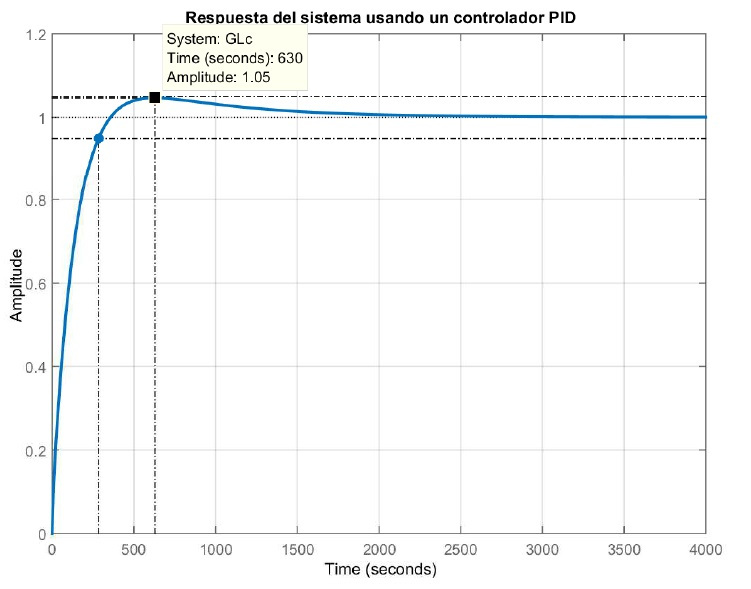
\includegraphics[width=110mm, height=80mm]{imagenes/capitulo4/4_6Resp_Lazo_Cerrado}
   \caption{Respuesta del sistema a una entrada escalón usando el PID diseñado}
   \label{4_6:resp_simulacion}
\end{figure}

\subsection{Discretizaci'on del controlador PID}\label{subsec:discretizacionPID}

	La discretización del controlador PID consiste en obtener la expresión matemática del controlador PID en tiempo discreto para que pueda ser implementado en un sistema digital. Para ello, se va a discretizar cada una de las acciones que definen al controlador PID y se agrupan las expresiones obtenidas en cada discretización. A continuación se detalla la discretización de cada acción:

\begin{itemize}
         \item\textbf{Discretizaci'on de la acci'on proporcional:} es la m'as f'acil de realizar ya que se basa en el muestreo de la se'nal de error.
	\begin{equation}\label{ecuacion_prop}
		\large m_{p}(n) =\left. K_{p} e(t) \right|_{t=kT_{s}} =  K_{p} e(kT_{s}) =   K_{p} e(n)
           \end{equation}
	\item\textbf{Discretizaci'on de la acci'on integral:} se basa en la discretizaci'on de la integral. Existen diferentes m'etodos para poder discretizarla (integraci'on hacia delante, integraci'on hacia atr'as, m'etodo de tustin...)\cite{PID}. Se ha decidido escoger el m'etodo de tustin ya que es una aproximaci'on m'as precisa y permite conservar la estabilidad del sistema en tiempo discreto.
	\begin{equation}\label{ecuacion_int}
	   \begin{split}
		 m_{i}(n) & = \left.  K_{i}\int_0^t e(t)dt \right|_{t=kT_{s}} =  K_{i}\sum_{k=1}^n  T_{s}\frac{e(kT_{s}) + e([k+1]T_{s})}{2} \\
                                     & = m_{i}(n-1) +  T_{s}\frac{e(kT_{s}) + e( [k+1]T_{s}\big)}{2} 
 	   \end{split}	
	\end{equation}
	 \item \textbf{Discretizaci'on de la acción derivativa:} se basa en la aplicaci'on del m'etodo de Euler hacia atr'as. De este modo, se consigue conservar la estabilidad.
            \begin{equation}\label{ecuacion_der}
		m_{d}(n)  =\left.  K_{d} \frac{de(t)}{dt} \right|_{t=kT_{s}}= K_{d} \frac{e(kT_{s}) - e([k-1]T_{s})}{T_{s}}
	\end{equation}
\end{itemize}

	Por tanto, la se'nal de control en el instante \textit{n} es la suma de las ecuaciones \ref{ecuacion_prop}, \ref{ecuacion_int} y \ref{ecuacion_der}. Para obtener una expresión más simplificada y fácil de implementar, se calcula la expresión de señal de control en \textit{n-1} y se hace la resta de la expresión en \textit{n} con la de \textit{n-1}. La expresión obtenida es la siguiente:
\begin{equation}\label{ecuacion4_6}
		m(n) = m(n-1) + q_{0} e(n) + q_{1} e(n-1) + q_{2} e(n-2)   
\end{equation}
	donde los coeficientes {$q_{0}$, $q_{1}$  y $q_{2}$ tienen las siguientes expresiones:\\
\begin{equation}\label{ecuacion4_7}
		q_{0} = \left( K_{p} + \frac{K_{d}}{T_{s}} +  \frac{K_{i}T_{s}}{2} \right) \quad q_{1} = \left( - K_{p} - \frac{2K_{d}}{T_{s}} +  \frac{K_{i}T_{s}}{2} \right)  \quad q_{2} = \frac{K_{d}}{T_{s}}
\end{equation}

	Para verificar que la discretización es válida, se ha simulado en MATLAB dicha discretización y se ha comparado con la respuesta de la figura \ref{4_6:resp_simulacion}. Dicha comparativa puede verse en figura \ref{4_7:discretizacionPID}. En dicha imagen se observa que la discretización se aproxima con bastante precisión a la respuesta continua.

\begin{figure}[h]
  \centering
  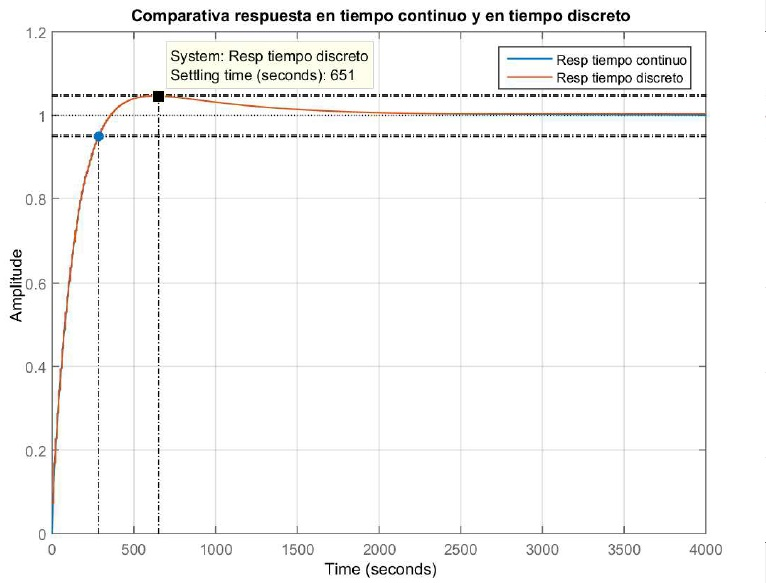
\includegraphics[width=110mm, height=71mm]{imagenes/capitulo4/4_7Resp_Lazo_Cerrado_Discreto}
   \caption{Respuesta del sistema a una entrada escalón con el PID discretizado}
   \label{4_7:discretizacionPID}
\end{figure}

\section{Bloque de generación de comandos}\label{sec:comandos}

	Este bloque se ha dividido en 2 subbloques para facilitar la implementación y modularidad. En la figura \ref{4_8:diag_generacion_comandos} se muestra un esquema de las entradas y salidas del bloque y los subbloques que lo componen.

\begin{figure}[htbp]
  \centering
  \includegraphics[width=100mm, height=26mm]{imagenes/capitulo4/4_8_Generacion_Comandos}
   \caption{Esquema del bloque de generaci'on de comandos}
   \label{4_8:diag_generacion_comandos}
\end{figure}

	El subbloque de \textbf{selección del comando} selecciona el \textit{setpoint}, a partir del valor de la se'nal de control y el rango de funcionamiento del sistema de refrigeraci'on, y selecciona el comando asociado. El subbloque de \textbf{modulación del comando} modula ese comando para que pueda ser interpretado por el sistema de refrigeraci'on. 

\subsection{Subbloque de selecci'on del comando}\label{subsec:seleccionComando}

Su función es seleccionar la temperatura del sistema de refrigeraci'on a partir del valor de señal de control y teniendo en cuenta el rango de valores de funcionamiento. Dicho rango es un conjunto finito de valores discretos con una separación fija entre valores consecutivos. Teniendo en cuenta esto, se va a aplicar el siguiente criterio para seleccionar la temperatura:

\begin{itemize}
\item\textbf{Se'nal de control igual o superior a la temperatura m'axima:} en este caso se escoge la temperatura m'axima de funcionamiento. 
\item\textbf{Se'nal de control entre la temperatura m'inima y m'axima:} se escoge la temperatura obtenida del resultado de redondear el valor de la se'nal de control al entero m'as pr'oximo.
\item\textbf{Se'nal de control igual o inferior a la temperatura m'inima:} en este caso se escoge la temperatura m'inima de funcionamiento. 
\end{itemize}

	Hay que tener en cuenta que el valor de la señal de control est'a expresado en mil'esimas, por lo que es necesario convertirlo a unidades para poder seleccionar la temperatura de forma adecuada.

	Después, una vez fijada la temperatura de funcionamiento, se selecciona el comando asociado a esa temperatura. Un comando es una secuencia de bits (0's y 1's) que representa un modo de funcionamiento que puede ejecutar el sistema de refrigeraci'on. 

	Hace unos a'nos, algunos miembros de \textit{GreenLSI} realizaron un proyecto denominado Pimote \cite{PIMOTE}. Este proyecto consist'ia en el dise'no e implementaci'on de un mando a distancia universal. En ese trabajo se utiliz'o como banco de pruebas el sistema de refrigeraci'on de la sala B039, que es el mismo que se utiliza en este trabajo, por lo que están disponibles sus comandos de funcionamiento. Cada uno de estos comandos est'a almacenado en un fichero de texto y siguiendo un determinado protocolo. 

	Se ha decicido utilizar los comandos usados en el proyecto Pimote y el protocolo que utilizan. Dicho protocolo es sencillo y en él están perfectamente delimitados cada uno de los campos que componen el comando. La única modificación que se va a hacer en este trabajo es convertir cada fichero a formato binario para facilitar su uso en el sistema de actuación.  En la figura \ref{4_9:protocolo_comando} se muestra el esquema del protocolo. 
\begin{figure}[h]
  \centering
  \includegraphics[width=140mm, height=18mm]{imagenes/capitulo4/4_9_Protocolo_Comandos}
   \caption{Protocolo de almacenamiento del comando}
   \label{4_9:protocolo_comando}
\end{figure}

\noindent A continuación se detallan cada uno de los campos del protocolo:

\begin{itemize}
     \item\textbf{Bytes de relleno:} son 6 bytes y est'an reservados por si fuera necesario incluir un campo nuevo en la cabecera o ampliar el tama'no de un campo ya definido.
     \item\textbf{Longitud del Payload:} est'a formado por 1 byte e indica el n'umero de bytes que ocupa el campo de datos del comando.
      \item\textbf{Periodo de bit:} est'a formado por 2 bytes y contiene el tiempo de bit del comando expresado en microsegundos.
      \item\textbf{Periodo de la portadora:} est'a formado por 1 byte y contiene el periodo de la portadora expresado en microsegundos. 
      \item\textbf{Payload:} su tamaño varía según el comando seleccionado. Contiene la orden o modo de funcionamiento del aire acondicionado.
\end{itemize}

\subsection{Subbloque de modulaci'on del comando}\label{subsec:modulacion}

	Se función es modular el comando que se envía al aire acondicionado para que el receptor pueda interpretarlo y ejecutar la orden. En este trabajo se va a usar una modulaci'on digital de amplitud usando como portadora una se'nal cuadrada de periodo T\_carrier. En la figura \ref{4_10:modulacion_bits} se muestra un esquema que representa la modulaci'on de la secuencia de bits `0101'.  A continuaci'on se describe el proceso de modulaci'on de cada bit: 

\begin{itemize}
    \item\textbf{Modulaci'on de un `1':} se transmite una se'nal cuadrada de frecuencia igual a la portadora y durante un tiempo igual al periodo de bit . 
    \item\textbf{Modulaci'on de un `0':} no se transmite nignuna se'nal durante un tiempo igual al periodo de bit. 
\end{itemize}

\begin{figure}[htbp]
  \centering
  \includegraphics[width=100mm, height=35mm]{imagenes/capitulo4/4_10_Modulacion_Bits}
   \caption{Ejemplo de modulaci'on de una secuencia de bits 0101}
   \label{4_10:modulacion_bits}
\end{figure}


\section{Bloque de transmisi'on}\label{sec:transmision}

	Su función es enviar el comando al sistema de refrigeraci'on. Para facilitar su implementación y modularidad, se ha dividido en 2 subbloques. En la figura \ref{4_11:diag_transmision} se muetra un esquema con sus entradas y salidas, así como de los subbloques que lo componen. 

\begin{figure}[htbp]
  \centering
  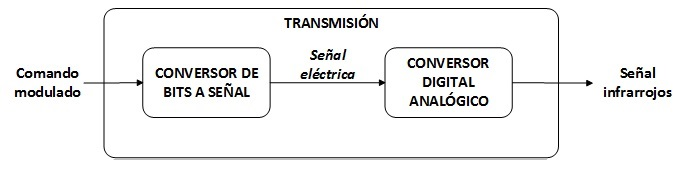
\includegraphics[width=140mm, height=32mm]{imagenes/capitulo4/4_11Bloque_Transmision}
   \caption{Diagrama del bloque de transmisi'on}
   \label{4_11:diag_transmision}
\end{figure}

	Primero, el \textbf{conversor de bits a señal} genera una señal eléctrica a partir de la secuencia de bits del comando y posteriormente, el \textbf{el circuito emisor de infrarrojos} la convierte en una señal de infrarrojos para que el sistema de refrigeración pueda interpretarla. A continuación se explican ambos subbloques con más detalle.

\subsection{Conversor de bits a señal}\label{subsec:conversor}

	Convierte la secuencia de bits que representa el comando modulado, en una se'nal el'ectrica. Dicha se'nal debe cumplir los requisitos de tiempo definidos en la modulaci'on (periodo de bit y periodo de la portadora). La transmisi'on de cada bit debe hacerse de forma síncrona para controlar el tiempo de bit y el tiempo de portadora. 

	Para ello, se ha decidido utilizar el protocolo SPI \textit{Serial Peripheral Interface}\cite{SPI}. Es un protocolo de comunicación serie síncrono que permite la transferencia de información entre un nodo principal llamado \textit{nodo maestro} y uno o varios nodos secundarios llamados \textit{nodos esclavos}. La transmisión de la información se realiza byte a byte, con un bit de parada entre transmisiones consecutivas. Un dispositivo SPI está formado por 4 pines:

\begin{itemize}
   \item\textbf{MOSI:} pin que se utiliza para enviar informaci'on a los nodos esclavos.
   \item\textbf{MISO:} pin que se utiliza para recibir informaci'on de los nodos esclavos. 
   \item\textbf{SCLK:} pin que emite una señal de reloj cuadrada, de frecuencia configurable, que se utiliza para sincronizar el envío de información entre los nodos.
   \item\textbf{CE:} pin que se utiliza para habilitar o deshabilitar la comunicaci'on con los nodos esclavos.
\end{itemize}

	La elecci'on de este protocolo se debe a que se puede controlar el tiempo de duraci'on de cada bit a trav'es de la se'nal SCLK. Por tanto, se puede realizar la modulaci'on correctamente y cumpliendo los requisitos de periodo de bit y periodo de portadora fijados en la etapa de modulaci'on. La interfaz SPI emite una señal eléctrica por el pin MOSI cuando se desear enviar el bit `1' ~ y no emite nada cuando se desea enviar el bit `0'. EL bit `1' ~ se asocia con un nivel de tensión alto (3,3 V o 5V), mientras que el bit `0' ~  se asocia con un nivel de tensión próximo a 0V.

\subsection{Circuito emisor de infrarrojos}\label{subsec:infrarrojos}

	Convierte la señal eléctrica en una señal de infrarrojos y la emite al sistema de refrigeración. En la figura \ref{4_12:emisor_IR} puede verse el esquema del circuito.

\begin{figure}[htbp]
  \centering
  \includegraphics[width=70mm, height=42mm]{imagenes/capitulo4/4_12_Emisor_IR}
   \caption{Esquema del circuito emisor de infrarrojos}
   \label{4_12:emisor_IR}
\end{figure}

	El circuito se basa en un diodo LED de infrarrojos (IRLED), un transistor BJT y un conjunto de resistencias. La resistencia R1 se usa para obtener la corriente de base que permite al transistor entrar en la región de saturación y la resistencia R2 se usa para polarizar el diodo en su punto de trabajo. El transistor trabaja en saturación y corte para que el diodo pueda generar la señal a transmitir. 

	El funcionamiento del transistor es el siguiente: cuando no se recibe tensión en la entrada del circuito (equivale a un '0'), el transistor entra en corte y la corriente de base y colector son muy próximas a 0. Al no haber corriente de colector, no circula corriente por el diodo, luego no emite señal. Sin embargo, cuando se recibe un nivel de tensión en la entrada (equivale a un '1'), el transistor entra en la región de saturación y circula corriente a través del diodo. El diodo convierte esa corriente en una señal de infrarrojos y la emite al sistema de refrigeración.

\section{Bloque de envío de datos}\label{sec:envioDatos}

	La función de este bloque es subir datos a la plataforma \textit{Graphite}. En la figura \ref{4_13:envio_datos} se muestra un esquema de sus entradas y salidas.

\begin{figure}[htbp]
  \centering
  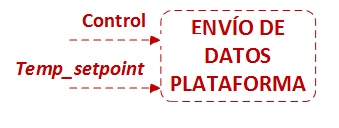
\includegraphics[width=70mm, height=30mm]{imagenes/capitulo4/4_13_Envio_Datos}
   \caption{Esquema del bloque de envío de datos}
   \label{4_13:envio_datos}
\end{figure}

	El bloque posee dos entradas, el dato de temperatura de control y el dato de \textit{setpoint}. Dichos valores se suben a la plataforma una vez se ha obtenido la temperatura de control y se ha seleccionado el \textit{setpoint}. El objetivo es poder visualizar el comportamiento de estas señales y así poder evaluar el comportamiento del actuador.

	Aunque no aparezca en el diagrama, en la fase de implementación se considerará la \textit{temperatura óptima} como otra entrada. El motivo es que en este trabajo  la \textit{temperatura óptima} va a estar fijada por el usuario y es necesario subir dicho valor a la plataforma. Una vez el actuador esté integrado con el sistema de optimización del CPD, dicho valor será leído desde la plataforma y no será necesario subirlo.

	Para poder subir los datos a la plataforma se ha tenido en cuenta los diferentes métodos disponibles para subir un dato, según  la documentación de \textit{Graphite} \cite{Graphite1}. Se ha usado un formato de texto plano para subir los datos, ya que presenta un formato sencillo y es fácil de implementar. Dicho formato presenta la estructura:

	\begin{verbatim}
	           <metric_path> <metric_value> <metric_timestamp>
	\end{verbatim}
 	
	El parámetro \textit{<metric\_path>} debe contener la dirección http y el puerto del servidor, junto con la ruta donde se va a escribir el dato. El parámetro \textit{<metric\_value>} debe contener el dato que se quiere subir a la plataforma. Por último, el parámetro \textit{<metric\_timestamp>} debe contener el instante de tiempo en el que se midió el dato.

	\chapter{Implementación}\label{cap:implementacion}

	En este capítulo se va a detallar la implementación, tanto a nivel hardware como software, del sistema de actuación y de cada uno de los bloques que lo componen.

	 El sistema de actuación se ha implementado en una Raspberry PI 2 model B, ya que dispone de un buen procesador, un puerto ethernet para conexión a internet, una buena memoria y varios puertos GPIO e interfaces, incluido SPI. Cada uno de los bloques del sistema de actuación está implementado mediante un programa software que estará alojado en la Raspberry PI, a excepción del circuito de infrarrojos cuya implementación es hardware. En la figura \ref{5_1:Hardware} se muestra la Raspberry PI utilizada.

\begin{figure}[htbp]
  \centering
  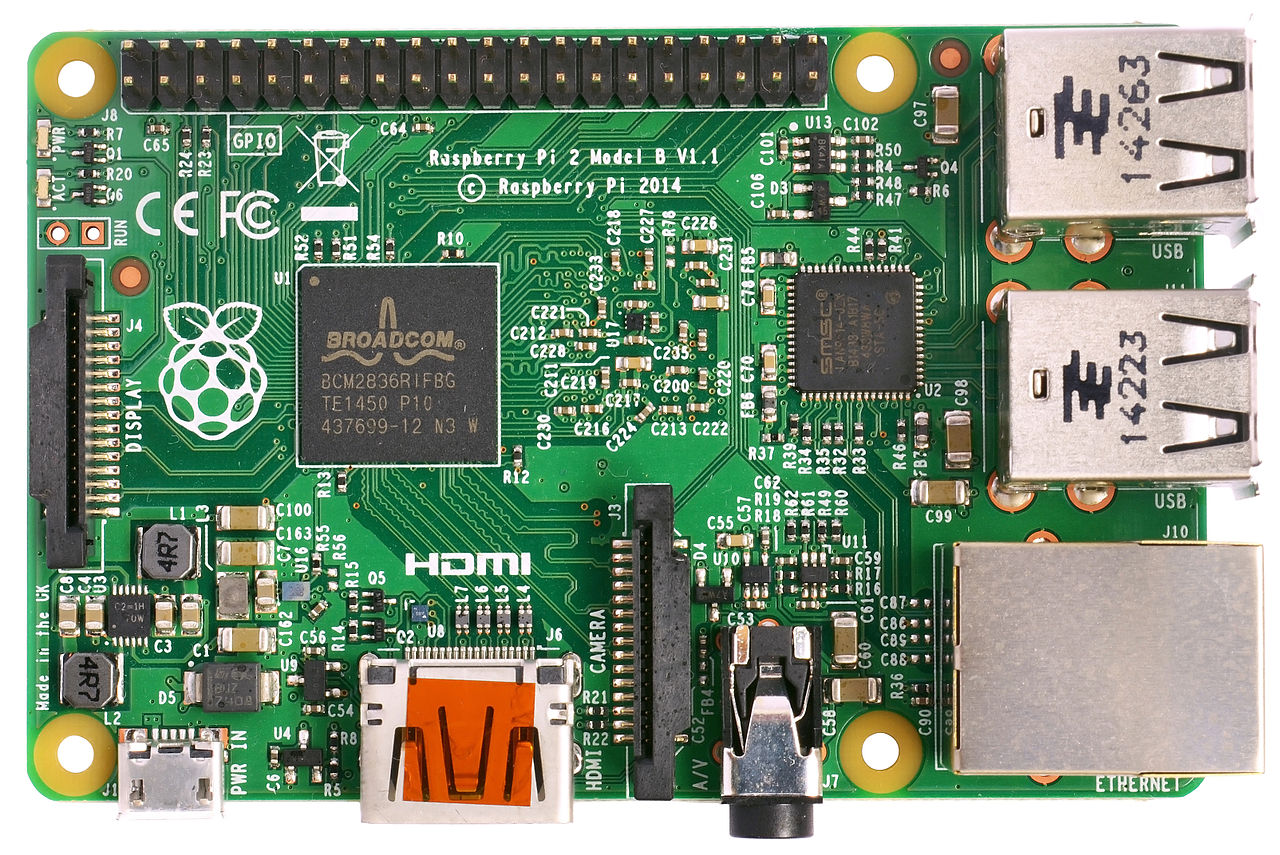
\includegraphics[width=70mm, height=40mm]{imagenes/capitulo5/5_1_RaspberryPI}
   \caption{Raspberry PI 2 model B}
   \label{5_1:Hardware}
\end{figure}

	El programa software está implementado en C ya que es un lenguaje de programación que posee características propias de los lenguajes de alto nivel y también permite manejar y gestionar la memoria y los puertos GPIO de la Raspbery PI de una forma sencilla.

	Cada bloque esta formado por un fichero \textbf{.c} y un fichero \textbf{.h}. El fichero \textbf{.c} contiene el código fuente de las funciones públicas y estáticas, así como las dependencias con otras librerías. El fichero \textbf{.h} contiene las macros y estructuras definidas, así como el prototipo de las funciones públicas implementadas en el fichero \textbf{.c}. En los siguientes apartados se detalla la implementación de cada bloque.

\section{Bloque de adquisición}\label{implementacion:adquisicion}

	La implementación de este bloque se encuentra en los ficheros \textbf{platformDown.c} y \textbf{platformDown.h}. Para facilitar dicha implementación, se han usado las librerías externas \textit{curl} \cite{curl} y \textit{jansson} \cite{jansson} para realizar las peticiones http y manejar los objetos en formato JSON respectivamente. A continuación se muestra la documentación de este modulo.

\noindent\Large\textbf{Macros definidas}\label{adquisición:macros}

\lstinputlisting[style=macros,firstline=1, lastline=10,texcl=true]{ficheros/platformDown.c}

\noindent\Large\textbf{Estructuras Definidas}\label{adquisición:estructuras}

\normalsize\textbf{struct objJSON}\label{estructuraobjJSON}
\lstinputlisting[style=estructura,firstline=15, lastline=21,texcl=true]{ficheros/platformDown.c}

\normalsize\textbf{struct temp\_leida}\label{estructuratempLeida}
\lstinputlisting[style=estructura,firstline=26, lastline=32,texcl=true]{ficheros/platformDown.c}

\noindent\Large\textbf{Funciones estáticas definidas}\label{adquisicion:functEstaticas}

\normalsize\textbf{escribir\_objeto()}\label{adquisicion:escribirObjeto}

\lstinputlisting[style=funcion,firstline=34, lastline=47,texcl=true]{ficheros/platformDown.c}

\noindent\Large\textbf{Funciones publicas definidas}\label{adquisicion:funPublicas}

\normalsize\textbf{solicitar\_objeto()}\label{adquisicion:solicitarObjeto}

\lstinputlisting[style=funcion,firstline=50, lastline=60,texcl=true]{ficheros/platformDown.c}

A conitnuación se incluye su pseudocódigo para facilitar su compresión.

\lstinputlisting[style=pseudocodigo,texcl=true]{ficheros/solicitar_objeto.c}

\normalsize\textbf{extraer\_temperatura()}\label{adquisicion:extraerTemperatura}

\lstinputlisting[style=funcion,firstline=63, lastline=72,texcl=true]{ficheros/platformDown.c}

A conitnuación se incluye su pseudocódigo para facilitar su compresión.

\lstinputlisting[style=pseudocodigo,texcl=true]{ficheros/extraer_temperatura.c}

\section{Bloque de comparación}\label{implementacion:comparacion}

	La implementación del bloque de comparación se encuentra en los ficheros \textbf{comparador.c} y \textbf{comparador.h}. Este módulo sólo dispone de la función \textit{calcular\_error()}. A continuación se incluye su documentación.

\textbf{calcular\_error()}\label{comparacion:calcularError}
\lstinputlisting[style=funcion,texcl=true]{ficheros/comparador.c}

\section{Bloque de control}\label{implementacion:control}

	La implementación de este bloque se encuentra en los ficheros \textbf{PID.c} y \textbf{PID.h}. A continuación se incluye la documentación de este módulo.

\noindent\Large\textbf{Macros definidas}\label{control:macros}

\lstinputlisting[style=macros,firstline=1, lastline=9,texcl=true]{ficheros/PID.c}

\noindent\Large\textbf{Funciones definidas}\label{control:funciones}

\normalsize\textbf{calcular\_tempcontrol()}\label{control:calcularTempControl}

\lstinputlisting[style=funcion,firstline=11, lastline=24,texcl=true]{ficheros/PID.c}

	La implementación del PID se basa en la expresión matemática del controlador PID discreto que aparece en la sección \ref{subsec:discretizacionPID}. El proceso consiste en ir calculando resultados parciales de esa fórmula y sumarlos todos para obtener el resultado final. El orden de operación es el siguiente:

\begin{enumerate}  
\addtolength{\itemsep}{-1mm}
\item Se calculan los productos y divisiones que conforman los coeficientes $q_{0}$, $q_{1}$ y $q_{2}$.
\item Se calculan los coeficientes $q_{0}$, $q_{1}$ y $q_{2}$.
\item Se calculan los productos de cada coeficiente con los valores de la señal de error.
\item Se suman los resultados de esos productos con el valor de la señal de control en el instante $n-1$, obteniendo el valor de la señal de control $m(n)$.
\end{enumerate}

	Esta función maneja números reales con una precisión de milésimas pero están expresados como números enteros. En el caso de las sumas y las restas no existen problemas de desbordamiento porque los números no son muy grandes. Sin embargo, en el caso de la multiplicación y división sí se manejan números muy grandes por lo que puede darse el caso de que al realizar este tipo de operaciones, se produzca desbordamiento u \textit{overflow} y el resultado generado sea incorrecto. Para solucionar este problema, se ha decidido implementar la multiplicación y división del siguiente modo:

\textbf{Implementación de la multiplicación}

	Supongamos 2 números reales A y B cada uno con una precisión de milésimas. A y B pueden ser expresados como la suma de su parte entera más su parte decimal.

\begin{equation*}
	\begin{aligned}
	A &= [A_{2}A_{1}A_{0},a_{1}a_{2}a_{3}] = \left( A_{2}A_{1}A_{0} + \frac{a_{1}a_{2}a_{3}}{1000}\right) \\
	B &= [B_{2}B_{1}B_{0},b_{1}b_{2}b_{3}]  = \left( B_{2}B_{1}B_{0} + \frac{b_{1}b_{2}b_{3}}{1000}\right)
	\end{aligned}
\end{equation*}

	Por tanto, el producto de A y B (A $\ast$ B) se obtiene realizando los subproductos de cada término de A por cada término de B. Dichos subproductos son:

\begin{equation*}
      \begin{aligned}
	 S_{p1} &= A_{2}A_{1}A_{0} \ast  B_{2}B_{1}B_{0} \rightarrow S_{p1} \text{(milésimas)} =  S_{p1} \ast 1000 \\
	 S_{p2} &= A_{2}A_{1}A_{0} \ast \left(\frac{b_{2}b_{1}b_{0}}{1000}\right) \rightarrow  S_{p2} \text{(milésimas)} = A_{2}A_{1}A_{0} \ast b_{2}b_{1}b_{0}\\
	 S_{p3} &= \left(\frac{a_{2}a_{1}a_{0}}{1000}\right) \ast B_{2}B_{1}B_{0} \rightarrow  S_{p3} \text{(milésimas)} = a_{2}a_{1}a_{0} \ast B_{2}B_{1}B_{0}\\
	 S_{p4} &= \left(\frac{a_{2}a_{1}a_{0}}{1000}\right) \ast \left(\frac{b_{2}b_{1}b_{0}}{1000}\right) \rightarrow  S_{p4} \text{(milésimas)}  = \left(\frac{a_{2}a_{1}a_{0} \ast b_{2}b_{1}b_{0}}{1000}\right) \\
      \end{aligned}
\end{equation*}

	Por tanto el resultado final es sumar cada uno de los subproductos expresado milésimas. De esta forma se evita el desbordamiento ya que la mayoría de los subrproductos generan el resultado directamente en milésimas sin necesidad de aplicar factores de conversión. Aquellos que no lo generan se les aplica el factor una vez se ha realizado el subproducto, lo que evita el manejo de números muy grandes. 

\noindent\textbf{Implementación de la división}

	Supongamos 2 números A y B cada uno con una precisión de milésimas. No se puede hacer la división con ambos números en las mismas unidades porque se pierde la parte decimal o sería necesario el uso de variables reales. Por tanto, es necesario multiplicar el dividiendo (en este caso A) por el factor de conversión de unidades a milésimas y dividir el resultado por el divisor (en este caso B). De este modo, el resultado obtenido es el mismo que si se hubiera hecho la división con números reales y truncado el resultado a milésimas. Además, se puede hacer la operación usando números enteros. A continuación se muestra un ejemplo de este proceso: 
\begin{equation*}
	\begin{aligned}
		A &= 13,135; \quad B = 4,328; \quad\rightarrow A/B = 3,0348 \sim 3,034 \text{ unidades} \rightarrow  3034 \text{ milésimas} \\
       		A &= 13,135 \ast 1000 ; \quad B = 4,328;    \quad\rightarrow A/B = 3034,8 \sim 3034 \text{ milésimas} 
	\end{aligned}
\end{equation*}
Hay que señalar que aunque este proceso se ha aplicado para números reales con una precisión de milésimas, es también aplicable para números reales con otra precisión aunque hay que tener en cuenta el tamaño de las variables que se estén usando.

\section{Bloque de generación de comandos}\label{sec:comandos}

	La implementación de este bloque y de los subbloques que lo componen se encuentra en los ficheros \textbf{comandos.c} y \textbf{comandos.h}. La implementación de cada subbloque se ha realizado en diferentes funciones para facilitar su modularidad. A continuación se incluye la documentación de este módulo.

\noindent\Large\textbf{Macros definidas}\label{comandos:macros}

\lstinputlisting[style=macros,firstline=1, lastline=40,texcl=true]{ficheros/comandos.c}

\noindent\Large\textbf{Estructuras definidas}\label{comandos:estructuras}

\normalsize\textbf{struct comando}\label{comandos:comando}

\lstinputlisting[style=estructura,firstline=43, lastline=49,texcl=true]{ficheros/comandos.c}

\normalsize\textbf{struct cmd\_modulado}\label{comandos:cmdModulado}

\lstinputlisting[style=estructura,firstline=51, lastline=59,texcl=true]{ficheros/comandos.c}

\noindent\Large\textbf{Funciones definidas}\label{comandos:funciones}

\normalsize Cada subbloque se ha implementado en diferentes funciones para facilitar su modularidad. A continuación se documentan las funciones de cada subbloque.

\subsection{Subbloque de selección del comando}\label{comandos:seleccion}

	La funcionalidad de este bloque se ha implementado mediante las funciones \textit{seleccionar\_setpoint()} y \textit{obtener\_comando()}. A continuación se documentan dichas funciones.

\normalsize\textbf{seleccionar\_setpoint()}\label{seleccion:setpoint}
\lstinputlisting[style=funcion,firstline=62, lastline=69,texcl=true]{ficheros/comandos.c}

\normalsize\textbf{obtener\_comando()}\label{seleccion:obtenerComando}
\lstinputlisting[style=funcion,firstline=72, lastline=81,texcl=true]{ficheros/comandos.c}

\subsection{Subbloque de modulación del comando}\label{comandos:modulacion}

Este subbloque se ha implementado con la función estática \textit{modular\_bit()} y la función \textit{modular\_comando()}. A continuación se documentan ambas funciones.

\normalsize\textbf{modular\_bit()}\label{modulacion:bit}
\lstinputlisting[style=funcion,firstline=84, lastline=96,texcl=true]{ficheros/comandos.c}

\normalsize\textbf{modular\_comando()}\label{modulacion:comando}
\lstinputlisting[style=funcion,firstline=99, lastline=110,texcl=true]{ficheros/comandos.c}

Como se ha mencionado en el apartado \ref{subsec:modulacion}, la modulación se realiza mediante la transmisión o no de una señal cuadrada de periodo $T_{carrier}$ y con una duración igual al tiempo de bit, dependiendo de sí se envía un '1'~ o un '0'. También se ha mencionado en la sección \ref{subsec:conversor} que se va a utilizar la interfaz SPI disponible en la raspberry PI para transmitir el comando al circuito emisor de infrarrojos. La modulación de cada bit se implementa del siguiente modo:

\begin{enumerate}
 \item \textbf{Modulación de un '0':} se implementa mediante una secuencia todo '0's.
 \item \textbf{Modulación de un '1':} se implementa mediante una secuencia de '1's y '0's alternados.
\end{enumerate}

	Ambas secuencias poseen la misma longitud y es el resultado de dividir el doble del periodo de bit por el periodo de la portadora (\textit{T\_carrier}). El motivo de dividir por el doble del periodo de bit es para conseguir la frecuencia deseada.

	Un factor que hay que considerar en la implementación de la modulación es que la interfaz SPI sólo permite transferencias byte a byte y que por cada byte transmitido, introduce un bit de parada. Por tanto, estos bits de parada deben ser considerados en la secuencia de modulación para que el comando modulado pueda ser interpretado por el aire acondicionado. Si no son considerados estos bits de parada, la modulación no se realiza correctamente y el aire acondicionado no podrá interpretar la orden.

	Por tanto, por cada 9 bits de la secuencia de modulación, debe ser descontado un bit de dicha secuencia, que será sustituido por el bit de parada. Este proceso se irá realizando de forma simultánea al proceso de generación del comando modulado. Sin embargo, este proceso depende de la posición de inicio de la secuencia de modulación de cada bit, ya que puede incluir más o menos bits de parada. 

\noindent Por tanto, el proceso de modulación consta de los siguientes pasos:

\begin{enumerate}
\item Se extrae de la cabecera el periodo de bit y el periodo de la portadora y se calcula la longitud de la secuencia de modulación de cada bit. 
\item Se calcula la longitud total de la secuencia de modulación del comando y los bits de parada que van a ser usado en dicha secuencia.
\item Se realiza la modulación de cada bit. Para ello, se tiene en cuenta el valor del bit, la posición de inicio de dicha secuencia dentro de una transferencia SPI, su posición final y el número de bits de parada que se van a usar en la modulación de ese bit.
\item Por último, una vez se ha realizado la modulación del comando, se comprueba que el número de bytes que ocupa dicha secuencia coincide con el número de bytes esperados y si es así devuelve un 0, indicando que la modulación se ha realizado correctamente. En caso contrario, devuelve -1.
\end{enumerate}

\section{Bloque de transmisión}\label{implementacion:transmision}

La implementación de este bloque es hardware y software. El conversor de bits a señal posee una implementación software, mientras que el circuito emisor de infrarrojos posee una implementación hardware. A continuación se detalla la implementación de ambos subbloques.

\subsection{Conversor de bits a señal}\label{sec:conversor}

La implementación de este subbloque se encuentra en los ficheros \textbf{spi.c} y \textbf{spi.h}. A continuación se incluye la documentación de este módulo.

\noindent\Large\textbf{Macros definidas}\label{conversor:macros}

\lstinputlisting[style=macros,firstline=1, lastline=13,texcl=true]{ficheros/spi.c}

\noindent\Large\textbf{Funciones definidas}\label{conversor:funciones}

\normalsize\textbf{transmitir\_comando()}

\lstinputlisting[style=funcion,firstline=16, lastline=23,texcl=true]{ficheros/spi.c}

	La función inicializa la librería pigpio y configura los puertos de la interfaz SPI. Después, crea un manejador SPI con el que realizar la transmisión y configura dicho dispositivo, incluyendo la frecuencia de bit. Por último, activa dicho dispositivo y transmite cada uno de los bytes del comando modulado. 

\subsection{Circuito emisor de infrarrojos}\label{conversor:circuito}

	Este circuito se ha implementado en una placa de inserción y se ha utilizado un diodo LED de infrarrojos LD271, un transistor BJT npn y 2 resistencias. Las características del circuito son las siguientes:\\ \\
           \textbf{Tensión de alimentación:} $V_{CC}=5V$. \\
	\textbf{Tensión y corriente del diodo:} $V_{D}=1,3V$ y $I_{D}=130mA$. \\
	\textbf{BJT en corte:} $I_{C} = I_{B} = 0$. \underline{Condición:} $V_{BE}<V_{\gamma E}$.\\ 
          \textbf{BJT en saturación:} $V_{BE} = V_{\gamma E}$, $V_{CE} = V_{CE(SAT)}$. \underline{Condiciones:} $I_{C}<\beta I_{B}$, $ I_{B}>0$.\\
           \textbf{Parámetros transistor:} $\beta=100$, $V_{CE(SAT)}=0,2V$ y $V_{\gamma E}=0,7V$. \\
           \textbf{Señal de entrada:} es una señal digital de valores $V_{HIGH}=3,3V$ y $V_{LOW}=0V$.

A continuación se muestra el análisis del circuito suponiendo que el transistor está en saturación. No es necesario hacerlo en corte porque en ese estado no circula corriente por el circuito y se alcanzaría dicho estado con cualquier valor de R1 y R2.
\begin{gather*} 
V_{R2} = V_{CC} - V_{D} - V_{CE(SAT)} = 5 - 1,3 - 0,2 = 3,5 V \\
\boxed{R2 = \frac{V_{R2}}{I_{D}} = 26,92 \Omega }\\ 
I_{B} > \frac{I_{C}}{\beta} = 1,3 mA  \quad \text{Se elige} \quad  I_{B}=16 mA\\
\boxed{R_{1}= \frac{V_{IN}-V_{BE(SAT)}}{I_{B}}=\frac{3,3-0,7}{0,016}=162,5 \Omega}
\end{gather*}
Por tanto, los valores de los componentes son: \fbox{$R_{1}=160\Omega \pm 5\%$  y $R_{2} = 27\Omega \pm 5\%$}

Por último, en la figura \ref{circuitoIR} se muestra el circuito de infrarrojos implementado. Hay que indicar que la resistencia $R_{1}$ se ha hecho conectando varias resistencias en serie que equivalen a su valor. 

\begin{figure}[htbp]
	\centering
	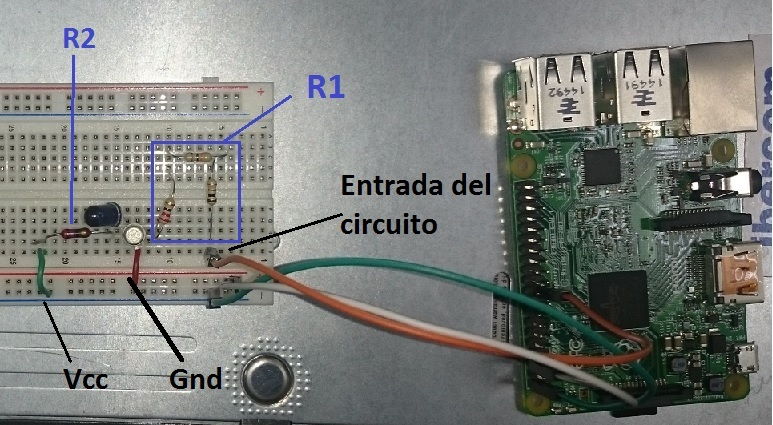
\includegraphics[width=115mm, height=50mm]{imagenes/capitulo5/circuitoIR}
   	\caption{Imagen del circuito de infrarrojos}
   	\label{circuitoIR}
\end{figure}

\section{Bloque de envío de datos}\label{implementacion:envioDatos}

La implementación de este bloque se encuentra en los ficheros \textbf{platformUp.c} y \textbf{platformUp.h}. Este módulo sólo contiene la función \textit{enviar\_datos()}. A continuación se incluye su documentación.

\lstinputlisting[style=funcion,texcl=true]{ficheros/platformUp.c}

\section{Ciclo de ejecución}\label{implemnetacion:actuador}

La implementación del ciclo de ejecución está en el fichero \textbf{actuador.c}. En este fichero se encuentra la función \textit{main()} que se encarga de realizar el ciclo del actuador y coordinar cada una de las etapas. A continuación se muestra el pseudocógido de dicha función.

\lstinputlisting[style=pseudocodigo,texcl=true]{ficheros/actuador.c}



	\chapter{Test y resultados}\label{cap:test}

	En este capítulo se detallan las pruebas realizadas para verificar el correcto funcionamiento del sistema de actuación. Estas pruebas se han llevado a cabo en el banco de pruebas descrito en el capítulo \ref{cap:bancopruebas}, ya que es un entorno real y adecuado para probar el funcionamiento del actuador.

	Las pruebas están orientadas a verificar el funcionamiento del actuador y comprobar que es capaz de controlar la temperatura de la sala y ajustarla al valor óptimo. El intervalo de temperaturas usado para hacer las pruebas es [18{$^\circ$}C - 24{$^\circ$}C], ya que este intervalo garantiza un correcto funcionamiento de la sala. Para realizar las pruebas, no se ha utilizado el dato proporcionado por el algoritmo de optimización, sino que dicho valor está fijado de forma manual. El objetivo es comprobar que el sistema consigue fijar la temperatura de la sala al valor óptimo y comprobar que funciona correctamente. Una vez se compruebe su funcionamiento, se procederá a su integración en el sistema de optimización. 

	El sensor de la sala tiene una precisión de $\pm$ 0,5{$^\circ$}C, luego éste es el mínimo ajuste de temperatura que puede hacer el actuador. Por otro lado, hay que tener en cuenta que el actuador debe poder realizar ajustes de temperatura  pequeños  (de $\pm$ 0,5{$^\circ$}C o $\pm$ 1,0{$^\circ$}C) y grandes ($\pm$ 3{$^\circ$}C o superior). 

	Por tanto, para comprobar que el actuador es capaz de controlar la temperatura y realizar ajustes tanto pequeños como grandes, se han hecho 4 tipos de pruebas:

\begin{enumerate}
	\item Subir directamente la temperatura de la sala en al menos 3{$^\circ$}C.
           \item Bajar directamente la temperatura de la sala en al menos 3{$^\circ$}C.
           \item Subir la temperatura de la sala con incrementos de 0.5{$^\circ$}C.
           \item Bajar la temperatura de la sala con decrementos de 0.5{$^\circ$}C.
\end{enumerate} 

	Hay que aclarar que con estas pruebas se pretende verificar el funcionamiento en las situaciones más complejas. Se supone que si el sistema funciona correctamente en los casos extremos, también funcionará correctamente en los casos intermedios. A continuación se muestra la tabla \ref{tabla6_1:pruebas} con las caracteristicas de cada prueba realizada. 

	Por claridad, este capítulo sólo se incluye una prueba de cada tipo. En el anexo \ref{Anexo:experimentos} se incluyen otras pruebas realizadas para comprobar el funcionamiento del actuador. Las conclusiones obtenidas de todos los experimentos (incluidos los del anexo), se muestran en este capítulo.

\begin{table}[h]
\centering
\scalebox{0.80}[0.90]{
	\begin{tabular}{| c | c | c | c |}
		\hline
		\textbf{Num Exp} & \textbf{Tipo exp} &\textbf{Experimento}  & \textbf{Parámetros PID}\\
		\hline \hline
			\textbf{1} & 1 &Subida de 20{$^\circ$}C a 24{$^\circ$}C  & $K_{p}=28$ $K_{i}=0,037$  $ K_{d}=300$\\
		\hline
			\textbf{2} & 3 &Subida de 20{$^\circ$}C a 24{$^\circ$}en pasos de 0.5{$^\circ$}C & $K_{p}=28$ $K_{i}=0,037$  $ K_{d}=300$ \\
		\hline
			\textbf{3} & 2 & Bajada de 24{$^\circ$}C a 21{$^\circ$}C & $K_{p}=28$ $K_{i}=0,037$  $ K_{d}=300$\\
		\hline
			\textbf{4} & 4 &Bajada de 24{$^\circ$}C a 22{$^\circ$}C en pasos de 0.5{$^\circ$}C & $K_{p}=28$ $K_{i}=0,037$  $ K_{d}=300$\\
		\hline	
\end{tabular}}
\label{tabla6_1:pruebas}\caption{Características de los experimentos realizados}
 \end{table}

\section{Resultados de las pruebas}\label{sec:resultados}
A continuación se muestran unas capturas de \textit{Graphite} que muestran los resultados obtenidos de los 4 primeros experimentos. En cada captura se representa la temperatura a la que se encuentra la sala (azul), el \textit{setpoint} (verde), y la temperatura óptima (rojo).

\begin{figure}[htbp]
\centering
\textbf{Experimento 1}\\
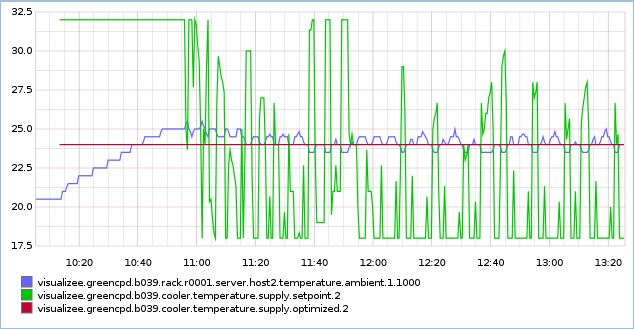
\includegraphics[width=120mm,height=85mm]{imagenes/capitulo6/experimento1}
\caption {Gráfica con los resultados del experimento 1}
\label{fig6_1:experimento1}
\end{figure}

\begin{figure}[htbp]
\centering
\textbf{Experimento 2}\\
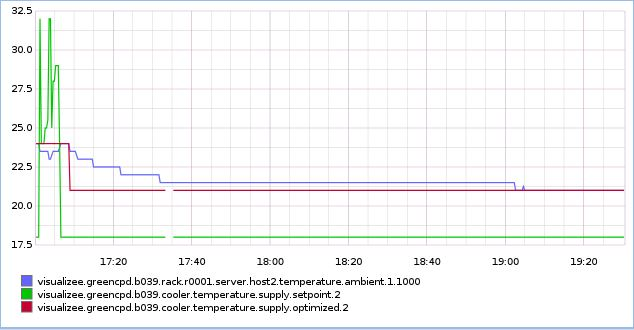
\includegraphics[width=120mm,height=85mm]{imagenes/capitulo6/experimento2}
\caption {Gráfica con los resultados del experimento 2}
\label{fig6_2:experimento2}
\end{figure}

\begin{figure}[htbp]
\centering
\textbf{Experimento 3}\\
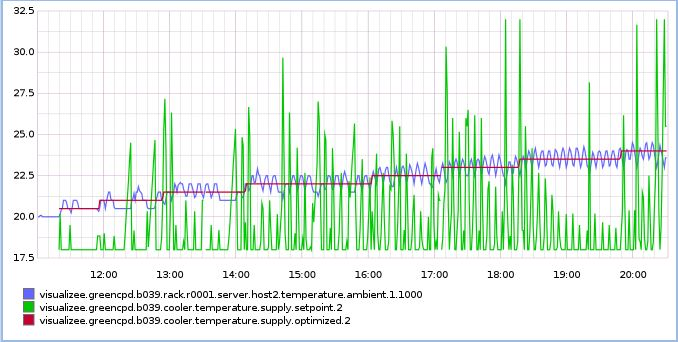
\includegraphics[width=120mm,height=85mm]{imagenes/capitulo6/experimento3}
\caption {Gráfica con los resultados del experimento 3}
\label{fig6_3:experimento3}
\end{figure}

\newpage

\begin{figure}[h]
\centering
\textbf{Experimento 4}\\
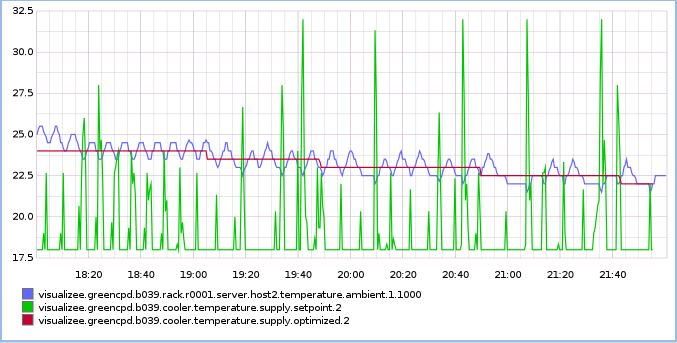
\includegraphics[width=120mm,height=85mm]{imagenes/capitulo6/experimento4}
\caption {Gráfica con los resultados del experimento 4}
\label{fig6_4:experimento4}
\end{figure}

	Hay que aclarar que en ninguna de las gráficas se ha incluido la señal de control. El motivo es que el controlador PID diseñado no tiene ningún mecanismo antiwindup, lo que hace que la señal de control en ocasiones tome valores demasiado grandes o pequeños que impiden visualizar correctamente el resto de señales. Se ha intentado añadir un mecanismo antiwindup al controlador pero no se han obtenido los resultados esperados. Por tanto, se ha decicido no incluir dicho mecanismo en este trabajo y se plantea la inclusión de este mecanismo como una linea futura. 

\section{Análisis de los resultados}\label{sec:análisis}
	Observando las gráficas de cada uno de los experimentos se comprueba que el actuador funciona correctamente y es capaz de controlar la temperatura del sistema y ajustarla al valor óptimo. Además, el actuador es capaz de ajustar la temperatura directamente o de forma gradual, lo que permite realizar ajustes de temperatura tanto pequeños como grandes. 

	 En todos los experimentos se observa un rizado en torno al valor óptimo. Este rizado es principalmente causado por la precisión del sensor. En principio, no supone un inconveniente a la hora de conseguir alcanzar la temperatura óptima, ya que suele ser pequeño y en la mayoría de las ocasiones coincide con la precisión del sensor.

	Hay que destacar el efecto windup que se ha producido en los experimentos 1, 5, 6, 8 y 11. El sistema de refrigeración dispone de un valor máximo y mínimo de funcionamiento y una vez que se alcanzan esos límites se satura. Sin embargo, el controlador PID diseñado es lineal por lo que el termino integral sigue aumentando y creciendo a pesar de que el sistema de refrigeración esté saturado. Cuando se supera la temperatura óptima, el error cambia de signo y el término integral comienza a compensarse aunque tardará un cierto tiempo como consecuencia del error acumulado en la etapa de subida. Esto provoca que se produzca una sobreoscilación, como se observa al inicio de los experimentos mencionados. 

	Este efecto es habitual que ocurra cuando se produce variaciones muy grandes de temperatura que se aproximan a la longitud del intervalo. Esta situación es poco probable que ocurra en un CPD, ya que es más habitual que el ajuste de temperatura sea gradual que ir moviéndose de extremo a extremo. A pesar de este efecto, se observa que el sobreajuste no es muy elevado y en poco tiempo la temperatura se estabiliza en torno a su valor óptimo.  Como ya se ha comentado, una posible mejora de este trabajo sería la implementación de un controlador PID con mecanismo antiwindup para corregir este problema.

	También se puede observar cómo influye la temperatura del exterior en la sala. En los experimento 2 y 7 se observa que la temperatura decae rápidamente pero a partir de un cierto valor, la temperatura tarda más tiempo en disminuir. Este efecto es provocado debido a la influencia de la temperatura exterior. El ciclo de evaporación se realiza en el exterior del edificio y si la temperatura exterior es elevada la eficiencia del ciclo de refrigeración se reduce y esto hace que tarde más tiempo en bajar la temperatura de la sala. Además, hay que recordar que el sistema de refrigeración del banco de pruebas es un aire acondicionado doméstico que no está diseñado para este tipo de salas, por lo que existe una limitación física que es ajena al sistema de actuación. Este efecto también se produce durante el invierno aunque de forma inversa. Esta es una de las razones por la que no se ha podido comprobar el funcionamiento del actuador en el caso de subir y bajar la temperatura de extremo a extremo.











	\chapter{Conclusiones y Líneas Futuras}\label{cap:conclusiones}

	En este cápitulo se exponen las conclusiones más importantes de este trabajo y cuáles son las bases para futuros trabajos relacionados.

\section{Conclusiones}

\noindent Una vez realizado el trabajo, las principales conclusiones que se extraen de él son:

\begin{itemize}

\item Se ha diseñado e implementado un sistema de actuación capaz de fijar la temperatura de una sala de servidores a un valor concreto, modificando la temperatura del sistema de refrigeración de dicha sala.

\item Se ha realizado un diseño modular y fácilmente extendible a otros entornos con diferentes plataforma de monitorización y visualización de datos, unidades de refrigeración o con diferentes politicas de control.

\item Se ha conseguido implementar un controlador PID sencillo que permite controlar la temperatura de la sala.

\item Se ha logrado un sistema de actuación autónomo, capaz de responder a los cambios de temperatura de manera dinámica y estable.

\item El sistema de actuación ha sido implantado en un entorno real (sala B039) y se integrado con la plataforma de monitorización y visualización \textit{Graphite}. Se ha verificado su funcionamiento en dicho entorno y se ha demostrado que el actuador funciona correctamente en un entorno real y consigue fijar la temperatura de la sala al valor deseado y para variaciones de temperatura tanto pequeñas como grandes.

\end{itemize}

\section{Lineas Futuras}

	Para terminar, se detallan las posibles acciones futuras que pueden llevarse a cabo, partiendo este trabajo:

\begin{itemize}

\item Diseñar el hardware propio del sistema de actuación e implementar el software en él. En este trabajo, se ha utilizado una Raspberry PI como soporte hardware. 

\item Analizar la posible implementación de otras políticas de control que permitan controlar la temperatura de la sala e implementarlas en el sistema de actuación de este trabajo para comprobar su funcionamiento. 

\item Optimizar el controlador PID existente, mediante un ajuste más fino de sus parámetros, añadir configuraciones que eviten el efecto windup o usar otro tipo de configuraciones PID más sofisticadas para así conseguir optimizar el funcionamiento del actuador.

\item Integrar el sistema de actuación en el sistema de optimización de CPDs diseñado por \textit{GreenLSI} y comprobar su funcionamiento en un entorno donde la temperatura óptima varía. En este trabajo, la temperatura óptima se elegía de manera arbitraria y era fijada por el usuario.

\item Extender el sistema a varias unidades de refrigeración. El sistema diseñado en este trabajo actúa sobre un único sistema de refrigeración. Es recomendable estudiar cómo se puede integrar el actuador en un entorno donde hay varias unidades de refrigeración y cómo se puede elaborar una respuesta coordinada que logre que la sala alcance la temperatura óptima.

\end{itemize}


	\chapter{Anexos} \label{Anexos}

\section{Anexo 1. Estimación de la función de transferencia}\label{ftrans}

	Este anexo está dividido en 2 partes: la primera parte incluye toda la información sobre el proceso de estimación de la función de transferencia descrito en el apartado \ref{subsec:caract_planta} y la segunda parte incluye el script de matlab elaborado para hacer este proceso.

\subsection{Proceso de estimación de la función de transferencia}

	Para estimar la función de transferencia se ha realizado un experimento que consiste en aplicar una señal de entrada escalón de 18{$^{\circ}$}C a 32{$^{\circ}$}C (para cubrir el rango de funcionamiento del sistema de refrigeración) y se ha medido la salida generada por dicho experimento. Este experimento se ha realizado 13 veces durante varios días y a diferentes horas para poder caracterizar mejor el comportamiento dinámico la planta.

	Para cada experimento se ha estimado la función de transferencia que mejor se ajusta a los datos generados en dicho experimento. Se han tenido en cuenta todas las combinaciones posibles de polos y ceros hasta orden 3. La selección de la función de transferencia se ha realizado en base al coeficiente de ajuste. 

	En la tabla \ref{tablaA1.1} se muestra la expresión matemática de la función de transferencia obtenida en cada experimento. Esta tabla sólo incluye la combinación que tiene un mayor coeficiente de ajuste. El resto de combinaciones se han descartado porque es poco probabile que una función que no se ajusta bien a sus propios datos pueda ajustarse mejor a los datos de los otros experimentos.

\newpage 

\begin{longtable}{| c | c | c |}
\hline
\textbf{Num exp} & \textbf{Función estimada} & \textbf{Coef ajuste} \\
\hline 
     &  &   \\
     &  \Large$ G(s) = \frac{6,624 \cdot 10^{-2}s^{2}+ 4,942 \cdot 10^{-4}s + 8,697 \cdot 10^{-7}}{ s^{3} + 0,5169 s^{2} + 3,318 \cdot 10^{-3}s + 1,123 \cdot 10^{-6}} $ &  \\
  1 &  & 91,3831\%  \\
     &  $ z_{1} = -4,6 \cdot 10^{-3},\quad z_{2} = -2,8 \cdot 10^{-3} $ &   \\
     &  $ p_{1} = -0,5104,\quad p_{2} = -6,1 \cdot 10^{-3},$ &  \\
     &  $ p_{3} = -3,583 \cdot 10^{-4}$ &   \\
     &  & \\
\hline
     &  &   \\
     &  \Large$ G(s) = \frac{8,686 \cdot 10^{-2}s+ 1,213 \cdot 10^{-4}}{ s + 1,592\cdot 10^{-4}} $ & \\
  2 &  & 85,5679\% \\
     &  $ z_{1} = -1,4 \cdot 10^{-3} $ &   \\
     &  $ p_{1} = -1.5924\cdot10^{-4} $ &  \\
     &  &   \\
\hline
     &  &   \\
     & \Large $ G(s) = \frac{4.382 \cdot 10^{-3}s+ 4.952\cdot 10^{-6}}{ s^{2} + 0.02972s + 6,397\cdot 10^{-6}} $ &  \\
  3 &  & 89,4146\%  \\
     &  $ z_{1} = -1,1 \cdot 10^{-3} $ &   \\
     &  $ p_{1} = -2,95 \cdot 10^{-2},\quad p_{2} = -2,167 \cdot 10^{-4} $ &  \\
     &  &   \\
\hline
     &  &   \\
     & \Large $ G(s) = \frac{4,976 \cdot 10^{-2}s^{2}+ 1.127 \cdot 10^{-3} + 1,805 \cdot 10^{-6}}{ s^{3} + 0.3519s^{2} + 7,369\cdot 10^{-3} + 2,314 \cdot 10^{-6}} $ \\
  4 &  & 91.4906\%   \\
     &  $ z_{1} = -2,09 \cdot 10^{-2},\quad z_{2} = -1,7 \cdot 10^{-3} $ &   \\
     &  $ p_{1} = -0,3296,\quad p_{2} = -2,20 \cdot 10^{-2},$ &  \\
     &  $ p_{3} = -3,189 \cdot 10^{-4} $ & \\
     &  &   \\
\hline
     &  &   \\
     &  \Large$ G(s) = \frac{2,033 \cdot 10^{-2}s^{2}+ 6.038 \cdot 10^{-4} + 8,775 \cdot 10^{-7}}{ s^{3} + 0.1792s^{2} + 4,498\cdot 10^{-3} + 1.191 \cdot 10^{-6}} $ &  \\
  5 &  & 88.7664\%  \\
     &  $ z_{1} = -2,82 \cdot 10^{-2},\quad z_{2} = -1,5 \cdot 10^{-3} $ &   \\
     &  $ p_{1} = -0,1490,\quad p_{2} = -2,99 \cdot 10^{-2}, $ &  \\
     &  $ p_{3} = -2,6754 \cdot 10^{-4} $ & \\
     &  &   \\
\hline
     &  &   \\
     &  \Large$ G(s) = \frac{8,432 \cdot 10^{-5}s + 1,697 \cdot 10^{-9}}{ s^{3} + 0,282s^{2} + 2,155\cdot 10^{-4} + 1.046 \cdot 10^{-14}} $ &  \\
  6 &  & 90,0349\%  \\
     &  $ z_{1} = -2,0124 \cdot 10^{-5}$ &   \\
     &  $ p_{1} = -0,2813,  p_{2} = -7,663\cdot 10^{-4}, $ &  \\
     &  $ p_{3} = -4,85 \cdot 10^{-11} $ & \\
     &  &   \\
\hline
\newpage
\hline
\textbf{Num exp} & \textbf{Función estimada} & \textbf{Coef ajuste} \\
\hline
     &  &   \\
     &  \large$ G(s) = \frac{8,62\cdot 10^{-10}}{ s^{3} + 1,277 \cdot 10^{-3}s^{2} + 2,333\cdot 10^{-6} + 1.109 \cdot 10^{-9}} $ & \\
  7 &  & 84,4719\%  \\
     &  $ p_{1} = - 3.57\cdot 10^{-4} + 0,0013i,\quad p_{2} = -3.57\cdot 10^{-4}  - 0.0013i, $ &  \\
     &  $ p_{3}=- 5,747 \cdot 10^{-4} $ &   \\
     &  & \\
\hline
     &  &   \\
     &  \large$ G(s) = \frac{7,439 \cdot 10^{-2}s + 1,308 \cdot 10^{-4}}{ s^{2} + 0.5104s^{2} + 1.612\cdot 10^{-4}} $ &  \\
  8 &  & 90,4214\%  \\
     &  $ z_{1} = -1,8 \cdot 10^{-3}$ &   \\
     &  $ p_{1} = -0,5101,\quad p_{2} = -3,1601 \cdot 10^{-4}$ &  \\
     &  &   \\
\hline
     &  &   \\
     &  \large$ G(s) = \frac{7.628 \cdot 10^{-2}s^{2}+ 7.03 \cdot 10^{-4}s + 9.769 \cdot 10^{-7}}{ s^{3} + 0.548s^{2} + 4,787\cdot 10^{-3} + 1.211 \cdot 10^{-6}} $  \\
  9 &  & 91.0543\%  \\
     &  $ z_{1} = -7,5 \cdot 10^{-3},\quad z_{2} = -1,7 \cdot 10^{-3} $ &   \\
     &  $ p_{1} = -0,5392,\quad p_{2} = -8,6 \cdot 10^{-3}, $ & \\
     &  $ p_{3}= -2,61 \cdot 10^{-4} $ &  \\
     &  &   \\
\hline
     &  &   \\
     &  \large$ G(s) = \frac{4,413 \cdot 10^{-7}s + 2,439 \cdot 10^{-9}}{ s^{3} + 8,157 \cdot 10^{-2}s^{2} + 1,603\cdot 10^{-5}s + 3,753 \cdot 10^{-9}} $ &  \\
10 &  & 84,86\%  \\
     &  $ z_{1} = -5,5 \cdot 10^{-3}$ &   \\
     &  $ p_{1} = -8,14 \cdot 10^{-2},\quad p_{2} =-9,825 \cdot 10 ^{-5} + 1,9097 \cdot 10^{-4}i,$ &  \\
     &  $ p_{3} = -9,825 \cdot 10 ^{-5} - 1,9097 \cdot 10^{-4}i, $  &   \\
     &  &  \\
\hline
     &  &   \\
     &  \large$ G(s) = \frac{0,5884s + 1,197 \cdot 10^{-3}}{ s^{3} + 4,457s^{2} + 4,228 s + 1,475 \cdot 10^{-3}} $ &  \\
11 &  & 89,8722\% \\
     &  $ z_{1} = -2,03 \cdot 10^{-3}$ &   \\
     &  $ p_{1} =-3,0877,   p_{2} = -1,3688, $ & \\
     &  $ p_{3} = -3,4898 \cdot 10^{-4} $ &  \\
\hline
     &  &   \\
 12 &  \large$ G(s) = \frac{2,868 \cdot 10^{-4}}{ s + 3,319 \cdot 10^{-4}} \quad p_{1} = -3,3186 \cdot 10^{-4} $ &  89,0861\%\\
     &  &  \\
\hline 
     &  &   \\
     &  \large$ G(s) = \frac{2,449 \cdot 10^{-10}}{ s^{3} + 9,255 \cdot 10^{-3}s^{2} + 4,247 \cdot 10^{-6} s + 2,603 \cdot 10^{-10}} $ & \\
13 &  & 91,05\%  \\
     &  $  p_{1} =-8,8 \cdot 10^{-3},  p_{2} = -4,0788 \cdot 10^{-4}, $ & \\
     &  $  p_{3} = -7,2718 \cdot 10^{-5} $ &  \\
\hline \\
\caption{Tabla con las funciones de transferencia estimadas}\label{tablaA1.1}
\end{longtable}

	Una vez determinada las función de transferencia mejor ajustada en cada experimento, se mide cómo se ajusta cada una de estas funciones a los datos generados por el resto de experimentos. En la tabla \ref{tablaA1.2} se muestra el coeficiente de ajuste de cada función con respecto a sus datos y a los datos de los otros experimentos. Se ha marcado en negro la función que presenta un mejor ajuste para cada experimento.

Analizando los datos de la tabla \ref{tablaA1.2}, se observa que en cada experimento se obtiene un mejor ajuste con los datos propios. El experimento que tiene un mayor coeficiente de ajuste es el número 4 con un valor del 91,4906\%. Sin embargo, puede verse en la tabla que los experimentos 6 y 13 tiene un coeficiente de ajuste medio superior al 80\% y que sus funciones tienen mejores coeficientes de ajuste que el resto. Además, el experimento 6 y el experimento 13 tienen unos coeficientes de ajuste propio de 90,0349\% y 91,05\% respectivamente, luego la variación con el experimento 4 es mínima. Por tanto, se decide que los experimentos 6 y 13 proporcionan una función de transferencia que se ajusta mejor a todos los experimentos. 

	Para decidir cúal de las 2 funciones se aproxima mejor, se va a calcular el error medio y el error máximo absoluto que tienen ambas funciones con respecto a los datos de cada experimento. Además, se van a representar los resultados obtenidos en un diagrama de pareto para visualizarlos mejor. 

	En la tabla \ref{tablaA1.2} puede verse el coeficiente de ajuste, el error cuadrático medio y el máximo error absoluto de ambos experimentos y en las figuras \ref{A1_1:pareto1} y \ref{A1_2:pareto2} se muestra un diagrama de pareto coeficiente de ajuste - error medio y un diagrama de pareto coeficiente de ajuste - error máximo  respectivamente. 

\begin{figure}[H]
  \centering
  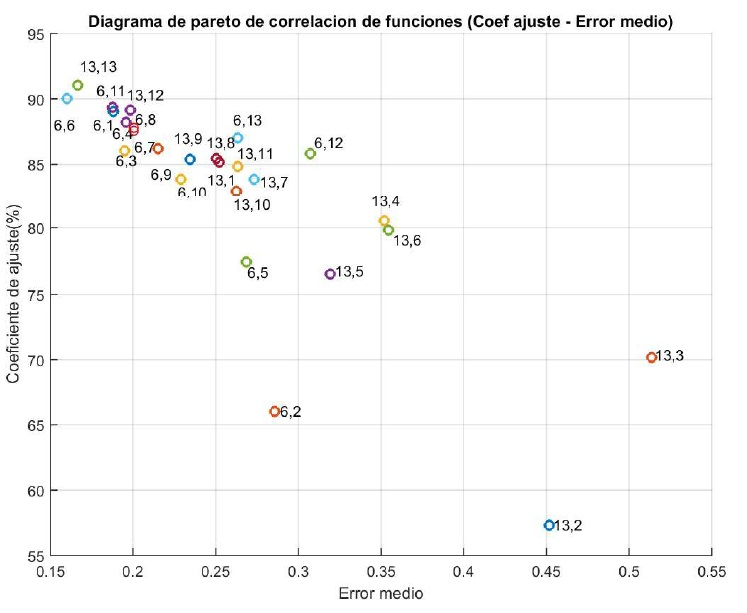
\includegraphics[width=115mm, height=85mm]{imagenes/anexo1/pareto1}
   \caption{Diagrama de pareto coef ajuste - error medio experimentos 6 y 13}
   \label{A1_1:pareto1}
\end{figure}

\begin{figure}[H]
  \centering
  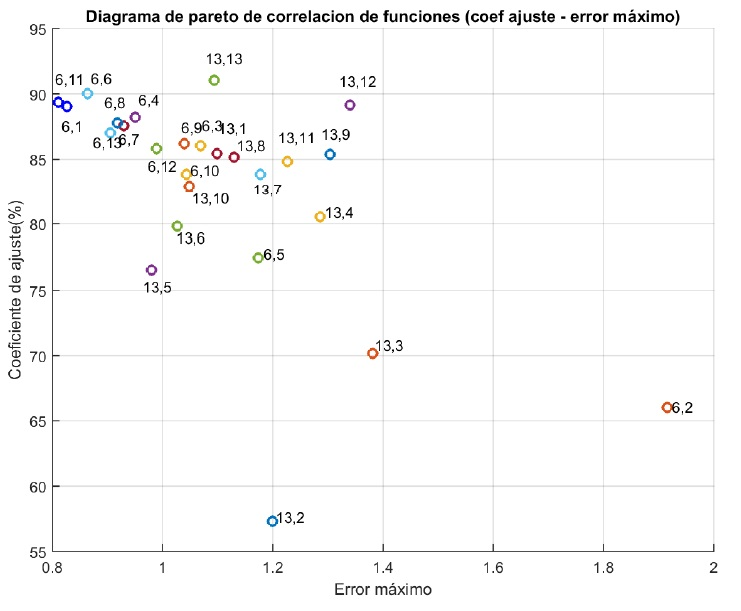
\includegraphics[width=115mm, height=85mm]{imagenes/anexo1/pareto2}
   \caption{Diagrama de pareto coef de ajuste - error máximo experimentos 6 y 13}
   \label{A1_2:pareto2}
\end{figure}

	Examinando dicha tabla se observa que el experimento 6 presenta mejores resultados medios con respecto al experimento 13 en los 3 parámetos. El experimento 6 tiene mejores valores en la mayoría de los experimentos con respecto al experimento 13. En ambos diagramas de pareto se observa que hay un mayor número de casos del experimento 6 situados en la parte superior izquierda de la figura, que se corresponde con un mayor coeficiente de ajuste y un menor error. Por otro lado, se observa que una gran parte de casos del experimento 13 se encuentra en la zona central de la figura, lo que implica que tienen un menor coeficiente de ajuste y un mayor error.

	Por tanto, se concluye que el experimento número 6 proporciona una función de transferencia estimada que se ajusta mejor a los datos de todos los experimentos  que el resto de experimentos y se decide que dicha función es la que mejor caracteriza el comportamiento dinámico de la planta. A continuación se muestra la expresión de dicha función de transferencia:

\begin{equation}\label{ecuacionA1_1}
           G(s) = \frac{8,4315 \cdot 10^{-5}s + 1,6968 \cdot 10^{-9}}{s^{3} + 0,2820s^{2} + 2,1553\cdot 10^{-4}s + 1,0462\cdot10^{-14}}
\end{equation} 

\begin{table}[p]\label{tablaA1.2}
\centering
\begin{sideways}
\scalebox{0.80}[0.90]{
	\begin{tabular}{| c | c | c | c | c | c | c | c | c | c | c | c | c | c | c |}
		\hline
		\multicolumn{15}{|c|}{Coeficiente de ajuste de cada experimento con las funciones estimadas en cada experimento} \\
		\hline
		\textbf{Num Exp} & \textbf{1} & \textbf{2} & \textbf{3} & \textbf{4} & \textbf{5} &\textbf{6} & \textbf{7} & \textbf{8} & \textbf{9} & \textbf{10} & \textbf{11} & \textbf{12} & \textbf{13} & \textbf{Media}\\
		\hline 
			\textbf{1} & \textbf{91,3831} &   7,7316 & 68,1859 & 91,3615 & 41,1466 & 90,1374  & 76,5276  & 74,2446  & 85,5091 &  83,1777 &  69,5568 & 30,6643 &  28,6190  & 62.2385 \\
		\hline
     			\textbf{2} & 46,4539 & \textbf{85,5679} & 63,6155 & 45,7268 & 74,5264 & 45,9584  & 33,6166  & 32,5180  & 40,0218 &  53,1230 &  30,0077 &   5,4745 &    3,0797  & 39,5102 \\
		\hline
			\textbf{3} & 73,0536 & 46,4246 & \textbf{89,4146} & 73,4109 & 77,5897 & 73,0610  & 57,8418  & 56,0292  & 66,0866 &  82,5248 &  52,3741 & 20,8814 &  19,2382  & 58,2096 \\
		\hline
			\textbf{4} & 90,3382 &   4,1194 & 67,5867 & \textbf{91,4906} & 41,9392 & 88,6594  & 76,7551  & 74,3276  & 85,7107 &  82,9944 &  69,6904 & 32,8622 &  31,3778  & 62,1968 \\
		\hline
			\textbf{5}& 58,2029  & 77,8641 & 69,5411 & 53,1426 & \textbf{88,7664} & 52,0389  & 36,8298  & 36,0635  & 43,4967 &  63,5883 &  32,9378 &  -4.4508 &  -9,3537  & 42.4918 \\
		\hline
			\textbf{6} & 89,0111  & 66,0086 & 86,0577 & 88,2092 & 77,4787 & \textbf{90,0349}  & 87,5776  & 87,7922  & 86,2082 &  83,8632 &  89,3537 & 85,8163 &  86,9912  & 84,5306 \\
		\hline
			\textbf{7} & 64,1301  &-29,3008 & 40,0983 & 68,4246 & -1.3793 & 67,5641  & \textbf{84,4719}  & 85,7168  & 75,2369 &  51,2921 &  84,5548 &  41,7830 & 38,3973  & 48,8765 \\
		\hline
			\textbf{8} & 75,5006  &-49,2439 & 33,4329 & 70,8841 & 10,6069& 67,0687  & 89,3440  & \textbf{90,4214}  & 78,5941 &  56,8271  &  88,3031 & 57,9744 & 58,9475  & 53,1866 \\
		\hline
			\textbf{9} & 89,6178  &-14,5296 & 54,8458 & 86,3504 & 39,7781& 83,3306  & 84,2851  & 81,8112  & \textbf{91,0543} &  77,8724  &  77,1474 & 48,0135 & 49,1641  & 63,1406 \\ 
		\hline
			\textbf{10} & 84,6609  & 67,2489 & 71,1708 & 84,5313 & 81,3005& 85,2595  & 84,9659  & 85,4456  & 84,5013  & \textbf{84,8600}   &  84,7497 &  63,8425 & 49,2469  & 77,2436 \\
		\hline
			\textbf{11} & 68,6527  &-60,2874 & 25,9336 & 64,1865 & -0.2220 & 60,4990  &85,8828  & 88,6983  & 72,3367  & 48,8204  &\textbf{89,8722}    & 61,1804  & 61,8088  & 48,1242 \\
		\hline
			\textbf{12} & 43,1090  &-134,0588 & -24,8806 & 26,2330 &-35,0181  & 21,6890 & 52,6691  & 58,4728   &35,7301  & 14,2683 &64,2494 & \textbf{89,0861} & 85,9484 & 17,3676 \\
		\hline
			\textbf{13} & 85,4331  & 57,3050 & 70,1803  & 80,5133 & 76,5364 & 79,8458 & 83,8308  & 85,1552 & 85,3857 & 82,9430 & 84,8552 &89,1679 &       \textbf{91,0500} &  80.0960\\
		\hline
                     \multicolumn{15}{|c|}{} \\
		\multicolumn{15}{|c|}{} \\
                     \hline
		\multicolumn{15}{|c|}{Coeficiente de ajuste de los experimentos 6 y13} \\
		\hline
			\textbf{Num Exp} & \textbf{1} & \textbf{2} & \textbf{3} & \textbf{4} & \textbf{5} &\textbf{6} & \textbf{7} & \textbf{8} & \textbf{9} & \textbf{10} & \textbf{11} & \textbf{12} & \textbf{13} & \textbf{Media}\\
		\hline 
			\textbf{6} & 89,0111  & 66,0086 & 86,0577 & 88,2092 & 77,4787 & \textbf{90,0349}  & 87,5776  & 87,7922  & 86,2082 &  83,8632 &  89,3537 & 85,8163 &  86,9912  & 84,5306 \\
		\hline
			\textbf{13} & 85,4331  & 57,3050 & 70,1803  & 80,5133 & 76,5364 & 79,8458 & 83,8308  & 85,1552 & 85,3857 & 82,9430 & 84,8552 &89,1679 &  \textbf{91,0500} &  80.0960\\
		\hline
			\multicolumn{15}{|c|}{} \\
		\hline 
			\multicolumn{15}{|c|}{Error cuadrático medio de los experimentos 6 y 13} \\
		\hline
			\textbf{Num Exp} & \textbf{1} & \textbf{2} & \textbf{3} & \textbf{4} & \textbf{5} &\textbf{6} & \textbf{7} & \textbf{8} & \textbf{9} & \textbf{10} & \textbf{11} & \textbf{12} & \textbf{13} & \textbf{Media}\\
		\hline 
			\textbf{6} & 0,1881  &  0,2859  &  0,1951  &  0,1956  &  0,2684  & \textbf{0,1599} & 0,2006  & 0,2006   &  0,2150  &  0,2291  &  0,1875   & 0,3074  &  0,2632  & 0,2280 \\
		\hline
			\textbf{13} & 0,2504    & 0,4515   &  0,5135   &  0,3518    & 0,3193  &  0,3546   & 0,2732    & 0,2523   &  0,2347   & 0,2625  & 0,2635  &  0,1985  &\textbf{0,1666} & 0,3105 \\
		\hline
			\multicolumn{15}{|c|}{} \\
		\hline 
			\multicolumn{15}{|c|}{Error máximo de los experimentos 6 y 13} \\
		\hline
		\textbf{Num Exp} & \textbf{1} & \textbf{2} & \textbf{3} & \textbf{4} & \textbf{5} &\textbf{6} & \textbf{7} & \textbf{8} & \textbf{9} & \textbf{10} & \textbf{11} & \textbf{12} & \textbf{13} & \textbf{Media}\\
		\hline 
			\textbf{6}  & 0,8270    & 1,9157    & 1,0695    & 0,9497    & 1,1739  & \textbf{0,8637}    & 0,9297    & 0,9183    & 1,0394    &1,0433   & 0,8114    & 0,9891    & 0,9058    & 1,0477 \\
		\hline
			\textbf{13} & 1,0991    & 1,1993    & 1,3817    & 1,2856    & 0,9804   & 1,0266   & 1,1769    & 1,1300    & 1,3033    & 1,0482   & 1,2258    & 1,3396    & \textbf{1,0941}    & 1,1830  \\
		\hline
\end{tabular}}
\end{sideways}
\caption{Coeficiente de ajuste de cada función con el resto de experimentos}
 \end{table}

\newpage	
\subsection{ Scripts de matlab para hacer la estimación}

	Este apartado incluye los scripts de matlab que se han diseñado para calcular la estimación de la función de transferencia. Se han diseñado 4 scripts.

\begin{itemize}
	\item\textbf{estimador.m:} este script se utiliza para extraer los datos de la plataforma y realizar la estimación de la función de transferencia para todas las combinaciones hasta orden 3.
	\item\textbf{seleccionarEstimacion.m:} este script se utiliza para seleccionar de cada experimento la función de transferencia que tiene un mejor coeficiente de ajuste.
	\item\textbf{analizador.m:} este script se utiliza para realizar la correlación entre todas las funciones de transferencia de todos los experimentos y seleccionar la función de transferencia que mejor se aproxima a todos los experimentos.
	\item\textbf{conv\_hora\_unix.m:} función que se utiliza para convertir la hora a formato unix. Esta función se utiliza en el script estimador.m.
\end{itemize}

	Para mayor claridad y debido a la longitud de estos scripts, se ha decidido no incluir el código en esta memoria. En su lugar, se ha habilitado un repositorio en github donde se pueden consultar estos scripts. La dirección http de este repositorio es la siguiente: \textbf{https://github.com/jccalvo/TFG.git}


 \newpage
    



	\section{Anexo 2: Otros experimentos}\label{Anexo:experimentos}

	Este anexo incluye algunos de los experimentos realizados en este TFG y que no han sido incluidos en el capítulo \ref{cap:test}. Estos experimentos están clasificados siguiendo los criterios definidos en dicho capítulo. Existe algún experimento que cubre un caso intermedio y por lo tanto, no ha podido ser clasificado. Sin embargo, también es interesante para evaluar el funcionamiento del actuador. En la siguiente tabla se muestra una relación de los experimentos que se incluyen en este anexo.

\begin{table}[h]
\centering
\scalebox{0.80}[0.90]{
	\begin{tabular}{| c | c | c | c |}
		\hline
		\textbf{Num Exp} & \textbf{Tipo exp} &\textbf{Experimento}  & \textbf{Parámetros PID}\\
		\hline 
			\textbf{5} & 1 &Subida de 19{$^\circ$}C a 24{$^\circ$}C  & $K_{p}=28$ $K_{i}=0,037$  $ K_{d}=300$\\
		\hline
			\textbf{6} & 1 &Subida de 19.5{$^\circ$}C a 23{$^\circ$}C  & $K_{p}=28$ $K_{i}=0,037$  $ K_{d}=300$ \\
		\hline
			\textbf{7} & 1 y 2 & Subida de 19.5{$^\circ$}C a 22{$^\circ$}C & $K_{p}=28$ $K_{i}=0,037$  $ K_{d}=300$\\
				       &          & y bajada de 22{$^\circ$}C a 18{$^\circ$}C & \\
		\hline
			\textbf{8} &  &  Subida de 21{$^\circ$}C a 23{$^\circ$}C  & $K_{p}=28$ $K_{i}=0,037$  $ K_{d}=300$\\
				       &  & y bajada de 23{$^\circ$}C a 21{$^\circ$}C & \\
		\hline	
			\textbf{9} & 3 & Subida de 19{$^\circ$}C a 23,5{$^\circ$}C en pasos de  0,5{$^\circ$}C & $K_{p}=28$ $K_{i}=0,037$  $ K_{d}=300$\\
		\hline
			\textbf{10} & 3 & Subida de 21.5{$^\circ$}C a 23,5{$^\circ$}C en pasos de  0,5{$^\circ$}C  & $K_{p}=28$ $K_{i}=0,037$  $ K_{d}=300$ \\
		\hline
			\textbf{11} & 1 y 4 &  Subida de 19.5{$^\circ$}C a 23{$^\circ$}C & $K_{p}=28$ $K_{i}=0,037$  $ K_{d}=300$\\
				         &          &  y bajada de 23{$^\circ$}C a 21,5{$^\circ$}C en pasos de 0,5{$^\circ$}C & \\
		\hline
			\textbf{12} & 3 & Subida de 19.5{$^\circ$}C a 21{$^\circ$}C en pasos de 0.5{$^\circ$}C& $K_{p}=28$ $K_{i}=0,037$  $ K_{d}=300$\\
		\hline	
\end{tabular}}
\label{tablaA2_1:pruebas}\caption{Características de los experimentos realizados}
 \end{table}

	En cada gráfica aparece la temperatura de la sala (azul), la temperatura óptima (rojo) y el setpoint (verde). No se ha incluido en ninguna gráfica la señal de control debido a que en ocasiones toma valores muy grandes o muy pequeños que impiden ver con claridad el resto de señales. A continuación se muestran las gráficas de los experimentos de la tabla \ref{tablaA2_1:pruebas}.

\newpage

\begin{figure}[H]
\centering
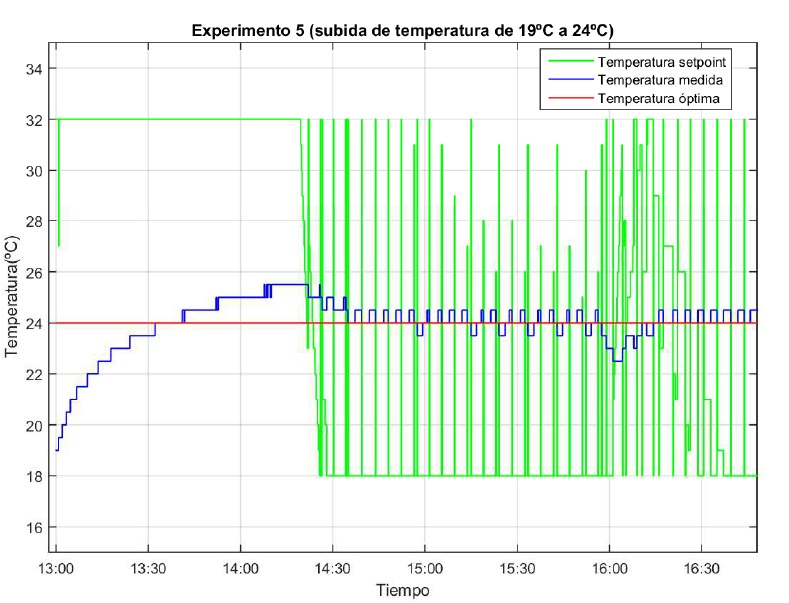
\includegraphics[width=130mm,height=95mm]{imagenes/anexo2/experimento5}
\caption {Gráfica con los resultados del experimento 5}
\label{figA2_1:experimento5}
\end{figure}

\begin{figure}[H]
\centering
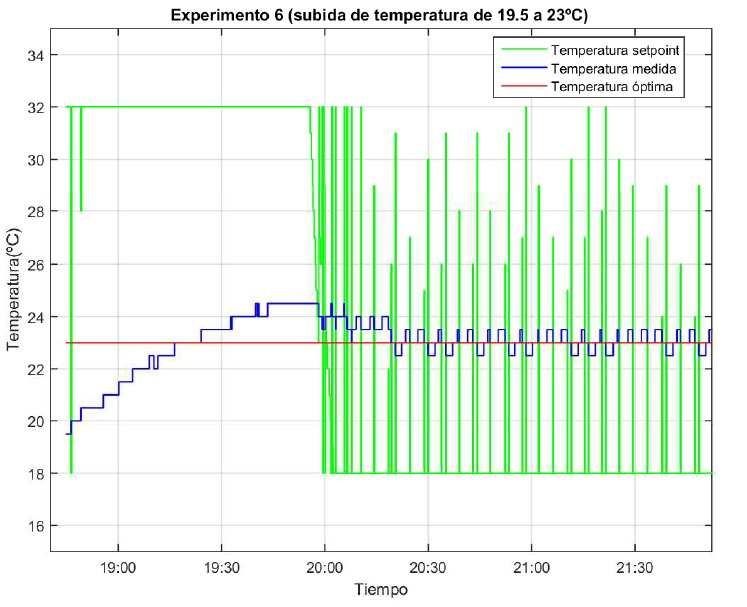
\includegraphics[width=130mm,height=95mm]{imagenes/anexo2/experimento6}
\caption {Gráfica con los resultados del experimento 6}
\label{figA2_2:experimento6}
\end{figure}

\begin{figure}[H]
\centering
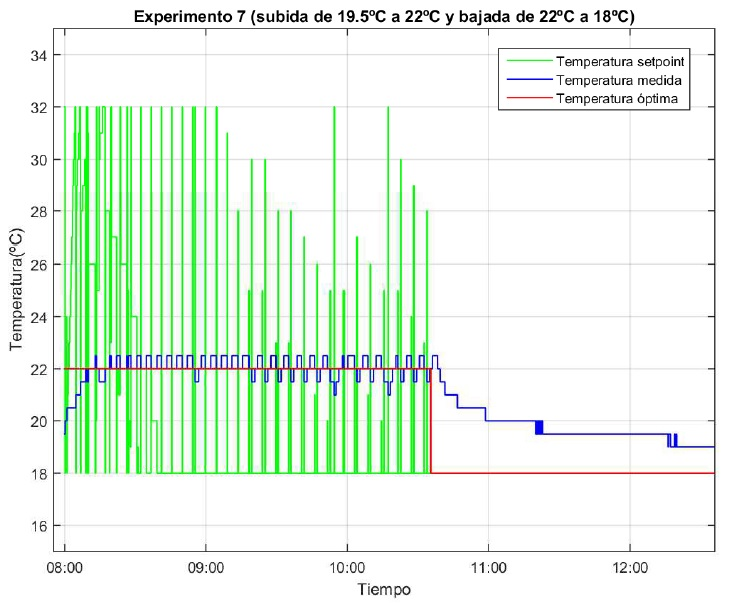
\includegraphics[width=130mm,height=95mm]{imagenes/anexo2/experimento7}
\caption {Gráfica con los resultados del experimento 7}
\label{figA2_3:experimento7}
\end{figure}

\begin{figure}[H]
\centering
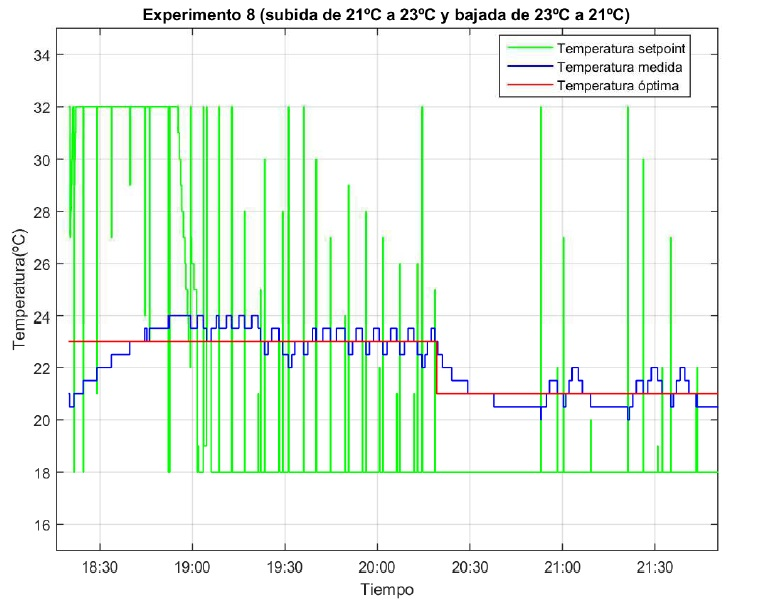
\includegraphics[width=130mm,height=95mm]{imagenes/anexo2/experimento8}
\caption {Gráfica con los resultados del experimento 8}
\label{figA2_4:experimento8}
\end{figure}

\begin{figure}[H]
\centering
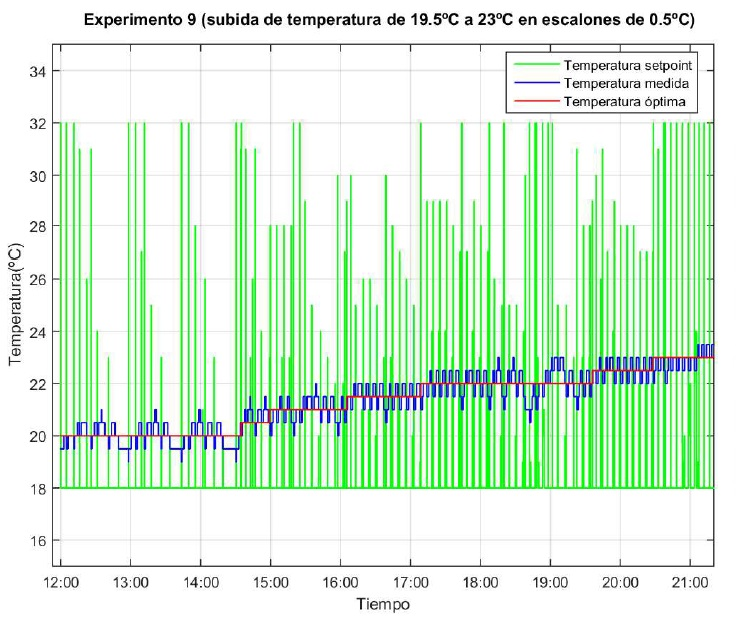
\includegraphics[width=130mm,height=95mm]{imagenes/anexo2/experimento9}
\caption {Gráfica con los resultados del experimento 9}
\label{figA2_5:experimento9}
\end{figure}

\begin{figure}[H]
\centering
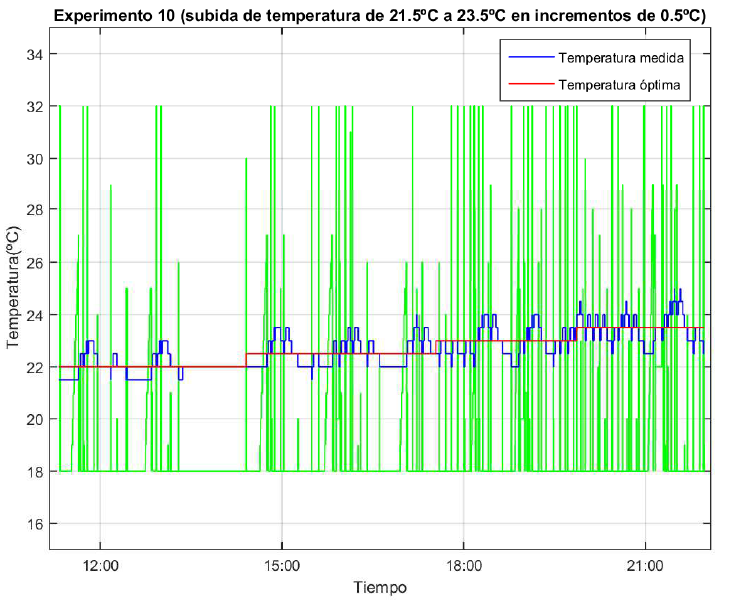
\includegraphics[width=130mm,height=95mm]{imagenes/anexo2/experimento10}
\caption {Gráfica con los resultados del experimento 10}
\label{figA2_6:experimento10}
\end{figure}

\begin{figure}[H]
\centering
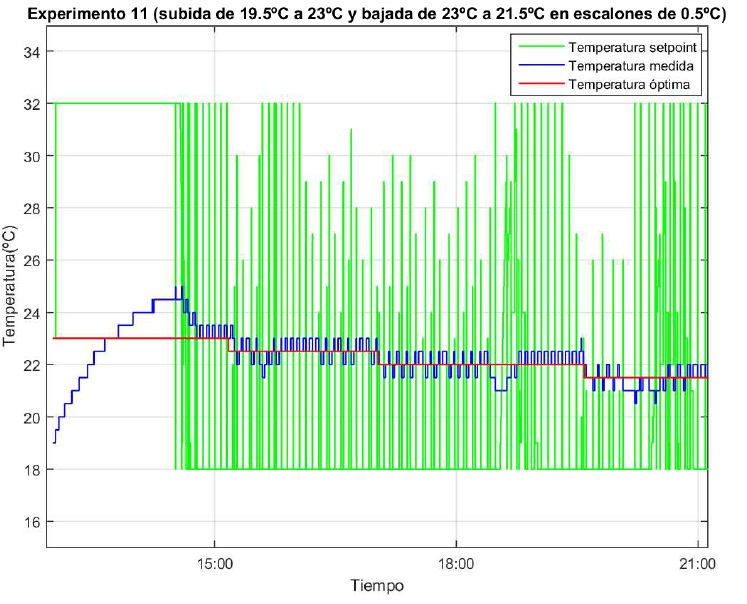
\includegraphics[width=130mm,height=95mm]{imagenes/anexo2/experimento11}
\caption {Gráfica con los resultados del experimento 11}
\label{figA2_7:experimento11}
\end{figure}

\begin{figure}[H]
\centering
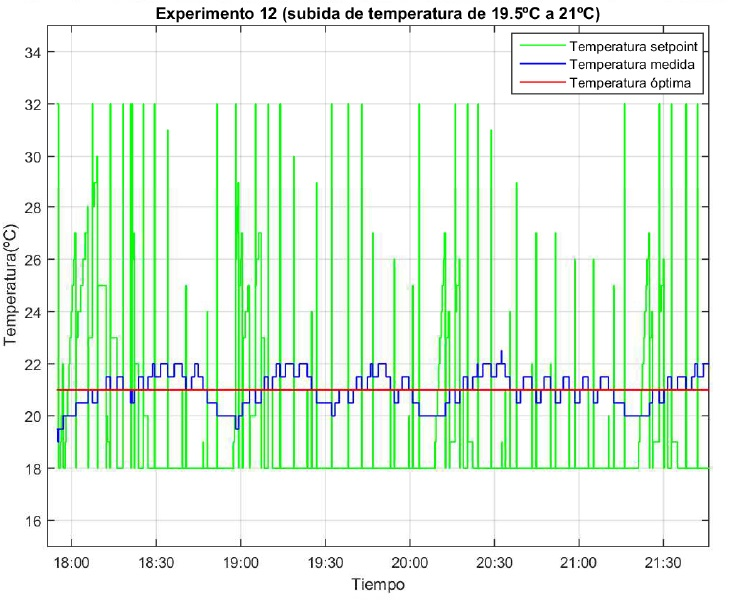
\includegraphics[width=130mm,height=95mm]{imagenes/anexo2/experimento12}
\caption {Gráfica con los resultados del experimento 12}
\label{figA2_8:experimento12}
\end{figure}

	\newpage
\section{Anexo 3: Script del controlador PID}\label{Anexo:scriptPID}

	En este anexo se incluye el script diseñado en matlab para ajustar el controlador PID y simular la respuesta del sistema ante ese controlador. El script es un único fichero denominado \textbf{PID.m}. En este script también se incluye el proceso de discretización del PID, usando la aproximación de tustin para evaluar si la discretización realizada es válida o no. A continuación se muestra el código de dicho script.

	Este script también se encuentra almacenado en el repositorio github indicado en el anexo \ref{ftrans}. La dirección http es: \textbf{https://github.com/jccalvo/TFG.git}

\lstinputlisting[style=matlab,texcl=true]{ficheros/controlador.m}
	\begin{thebibliography}{x}

	\bibitem{EMC} EMC corporation e IDC (international data corporation),
	\textit{``The digital universe of opportunities"}, 2014. \url{https://www.emc.com/collateral/analyst-reports/idc-digital-universe-2014.pdf}

	\bibitem{yole} M. Grao Txapartegi y Dr. Eric Mounier. 
	\textit{``Data Center Technologies. New Technologies and Architectures for Efficient Data Centers"}, Yole Développement, 2015. \url{http://www.i-micronews.com/images/Flyers/Power/Yole_New_Technologies_and_Architectures_for_Efficient_Data_Centers_Flyer_web.pdf}

	\bibitem{consumo1} EYP Mission Critical Facilities Inc., New York, 2011.

	\bibitem{consumo2} Rychard L. Sawyer, 
	\textit{``Calculating power requirements for data centers"}, APC y Schneider Electric, 2011. \url{http://www.apc.com/salestools/VAVR-5TDTEF/VAVR-5TDTEF_R1_EN.pdf}

	\bibitem{PUE} V. Avelar, D. Azevedo y A. French.
		\textit{``Pue: A comprehensive examination of the metric"}, 2014. \url{ https://datacenters.lbl.gov/sites/all/files/WP49-PUE\%20A\%20Comprehensive\%20Examination\%20of\%20the\%20Metric_v6.pdf}

	\bibitem{ITEfficiency} M. Zapater Sancho, P. Arroba García, J. M. Moya Fernández y Z. Bankovic. 
		\textit{``A state-of-the-art on energy eficiency in today's datacentres: Researcher's contributions and practical approaches"}, Vol. XII, Oct 2011. 

	\bibitem{DVFS} P. Chauhan y M. Gupta.
		\textit{``Energy Aware Cloud Computing Using Dynamic Voltage Frecuency Scalling"}, International Journal of Computer Science And Technology (IJCST), Vol 5, Issue 4, pp 195-199, Oct-Dec 2014. \url{ http://www.ijcst.com/vol54/2/49-Pooja-Chauhan.pdf}

	\bibitem{DPM} Silicon Valey Leadership Group,
		\textit{"Dynamic Power Management: Adjusting Data Center Capacity in Real-Time Energy Efficient Data Center Demonstration Project"}, 2009. \url{ http://svlg.org/wp-content/uploads/2012/12/PowerAssure_cs.pdf}

	\bibitem{VM} R. Buyya, A. Beloglazov y J. Abawajy. 
		\textit{``Energy-Efficient Management of Data Center Resources for Cloud Computing: A Vision, Architectural Elements, and Open Challenges"}, PDPTA, 2010. \url{https://pdfs.semanticscholar.org/65f3/92ea232878e416b077605427ff62d7fe0677.pdf}

	\bibitem{FreeCooling} Hainan Zhang, Shuangquan Shao, Hongbo Xu, Huiming Zou y Changqing Tian. 
	\textit{``Free cooling in a data centers: A review"}, Renewable and Sustainable Energy Reviews 35, pp 171-182, 2014. \url{ http://ac.els-cdn.com/S1364032114002445/1-s2.0-S1364032114002445-main.pdf?_tid=5780469c-30ef-11e7-bdaa-00000aab0f26&acdnat=1493919198_8346bfe1c779548bcc2e857ac03500bc} 

	\bibitem{OverCooling} Dan Hoffman.
		  \textit{``10 Techniques for improving data center power efficiency"}, Net app vision paper, Nov 2007. \url{http://www.uk.insight.com/content/dam/insight/EMEA/uk/shop/netapp/netappimproving-data-center-power-efficiency.pdf}

	\bibitem{cfugas} Y. Xie y W. L. Hung. 
		 \textit{``Temperature-aware task allocation and scheduling for embedded multiprocessor systems-on-chip (mpsoc) design"}, Journal of VLSI signal processing systems for signal, image and video technology, vol. 45, no. 3, pp. 177-189, 2006.

	\bibitem{GreenLSI} GreenLSI. \url{http://www.greenlsi.die.upm.es}

	\bibitem{RespConj} M. Zapater, J. L. Ayala y J. M. Moya. 
	           \textit{``Greendisc: a hw/sw energy optimization framework in globally distributed computation"}.  Ubiquitous Computing and Ambient Intelligence, pp 1-8, 2012. \url{http://oa.upm.es/16826/1/INVE_MEM_2012_137570.pdf}

	\bibitem{Monitorizacion} J. Pagan Ortiz, M. Zapater Sancho, O. Cubo, P. Arroba García, V. Martín Ayuso y J. M. Moya. 
	     \textit{A cyber-physical approach to combined hw-sw monitoring for improving energy eciency in data centers},  2013. \url{http://oa.upm.es/29886/1/INVE_MEM_2013_167142.pdf}

	\bibitem{Modelos} \textsc{M. Zapater}, \textsc{O. Tuncer}, \textsc{J. Ayala}, \textsc{J. Moya}, \textsc{K. Vaidyanathan}, \textsc{K. Gross} and \textsc{A. Coskun}. 
	      \textit{``Leakage-aware cooling management for improving server energy efficiency"}, IEEE Transactions on Parallel and Distributed Systems, vol 26, Issue:10, pp 2764-2777, oct 2015. 

	\bibitem{Esquema} Patricia Arroba, Jose M. Moya, Jose L. Ayala y Rajkumar Buyya.
	       \textit{``Proactive Power and Thermal Aware Optimizations for Energy-Efficient Cloud Computing"},  Design automation and test in europe (DATE), 2016. 

	\bibitem{control1} Katsuhiko Ogata. \textit{``Ingeniería de control moderna"}, Ed Pearson Education, 5º edición, 2010.

	\bibitem{control2} Benjamin C. Kuo. \textit{``Sistemas de control automático"}, Ed Prentice Hall, 7º Edición, 1996.
	       
	\bibitem{control3} Karl J. Astrom y Tore Hagglund. \textit{``Control PID avanzado"}, Ed Pearson Education, 2009. 

	\bibitem{PID} Bogdan M. Wilamoswski \& J. David Irwin. \textit{``The Industrial Electronics Handbook: Control and Mechatronics"}, 2º edition, CRC Press, 2011.
	
	\bibitem{fabricante1} Fabricante de controladores Omrom. \url{https://www.ia.omron.com/support/guide/53/introduction.html}

	\bibitem{fabricante2} Fabricante de controladores Omega. \url{http://www.omega.com/prodinfo/temperaturecontrollers.html}

	\bibitem{fabricante3} Fabricante de controladores Coulton. \url{http://www.coulton.com/QandA_controller}

	\bibitem{fabricante4} Fabricante de controladores Imopc. \url{http://www.imopc.es/content.php?p=spotlight_TempControl&lang=ES}

	\bibitem{Graphite1} Documentaci'on \textit{Graphite}. \url{http://graphite.readthedocs.io/en/latest/index.html}
	
	\bibitem{PIMOTE} Sara Álvarez Vinagre y Alfredo Tendero Casanova.
	\textit{Memoria proyecto Pimote SDG2}, GreenLSI, Departamento de Ingeniería Electrónica (DIE), Universidad Politécnica de Madrid, 2013.

           \bibitem{SPI} Protocolo de comunicación SPI. \url{http://www.i-micro.com/pdf/articulos/spi.pdf}

	\bibitem{curl} Librería \textit{curl} para peticiones HTTP en C. \url{https://curl.haxx.se/libcurl/}

	\bibitem{jansson} Librería \textit{jansson} para manejar objetos JSON en C. \url{https://jansson.readthedocs.io/en/2.10/}

\end{thebibliography}


\end{document}
